\documentclass[dissertation,copyright]{uathesis}
\usepackage[]{graphicx}\usepackage[]{color}
%% maxwidth is the original width if it is less than linewidth
%% otherwise use linewidth (to make sure the graphics do not exceed the margin)
\makeatletter
\def\maxwidth{ %
  \ifdim\Gin@nat@width>\linewidth
    \linewidth
  \else
    \Gin@nat@width
  \fi
}
\makeatother

\definecolor{fgcolor}{rgb}{0.345, 0.345, 0.345}
\newcommand{\hlnum}[1]{\textcolor[rgb]{0.686,0.059,0.569}{#1}}%
\newcommand{\hlstr}[1]{\textcolor[rgb]{0.192,0.494,0.8}{#1}}%
\newcommand{\hlcom}[1]{\textcolor[rgb]{0.678,0.584,0.686}{\textit{#1}}}%
\newcommand{\hlopt}[1]{\textcolor[rgb]{0,0,0}{#1}}%
\newcommand{\hlstd}[1]{\textcolor[rgb]{0.345,0.345,0.345}{#1}}%
\newcommand{\hlkwa}[1]{\textcolor[rgb]{0.161,0.373,0.58}{\textbf{#1}}}%
\newcommand{\hlkwb}[1]{\textcolor[rgb]{0.69,0.353,0.396}{#1}}%
\newcommand{\hlkwc}[1]{\textcolor[rgb]{0.333,0.667,0.333}{#1}}%
\newcommand{\hlkwd}[1]{\textcolor[rgb]{0.737,0.353,0.396}{\textbf{#1}}}%
\let\hlipl\hlkwb

\usepackage{framed}
\makeatletter
\newenvironment{kframe}{%
 \def\at@end@of@kframe{}%
 \ifinner\ifhmode%
  \def\at@end@of@kframe{\end{minipage}}%
  \begin{minipage}{\columnwidth}%
 \fi\fi%
 \def\FrameCommand##1{\hskip\@totalleftmargin \hskip-\fboxsep
 \colorbox{shadecolor}{##1}\hskip-\fboxsep
     % There is no \\@totalrightmargin, so:
     \hskip-\linewidth \hskip-\@totalleftmargin \hskip\columnwidth}%
 \MakeFramed {\advance\hsize-\width
   \@totalleftmargin\z@ \linewidth\hsize
   \@setminipage}}%
 {\par\unskip\endMakeFramed%
 \at@end@of@kframe}
\makeatother

\definecolor{shadecolor}{rgb}{.97, .97, .97}
\definecolor{messagecolor}{rgb}{0, 0, 0}
\definecolor{warningcolor}{rgb}{1, 0, 1}
\definecolor{errorcolor}{rgb}{1, 0, 0}
\newenvironment{knitrout}{}{} % an empty environment to be redefined in TeX

\usepackage{alltt}
\newcommand{\SweaveOpts}[1]{}  % do not interfere with LaTeX
\newcommand{\SweaveInput}[1]{} % because they are not real TeX commands
\newcommand{\Sexpr}[1]{}       % will only be parsed by R


%\documentclass[dissertation,CC-BY]{uathesis}
%\documentclass[dissertation,CC-BY-SA]{uathesis}
%documentclass[dissertation,CC-BY-ND]{uathesis}
%\documentclass[thesis]{uathesis}
%\documentclass[document]{uathesis}

% Package Usage
% These are the packages that we need
\usepackage{booktabs}
\usepackage{graphicx}
\usepackage{natbib}			% natbib is available on most systems, and is
					% terribly handy.
					
%May need to remove! Trying to fix nocite{*} biblography problem:
					% If you want to use a different Bibliography package, 
					% you should be able to, just change this
					% and the \bibliographystyle command below.  Be warned
					% that you may need to do a little hacking to get
					% the REFERENCES item to show up in your TOC.

% Compatibility with the AASTEX package 
% of the American Astronomical Society.
%\usepackage{deluxetable}		% Allows use of AASTEX deluxe tables
%\usepackage{aastex_hack}		% Allows other AASTEX functionality.

% These are other packages that you might find useful.
% For controlling the fonts, see
% http://www.math.uiuc.edu/~hartke/computer/latex/survey/survey.html
% The following is a nice font set:
%\usepackage{mathtime}			% Times for letters; Belleek math.
%
\usepackage{wrapfig}

\newenvironment{lydiawrapfigure}
 {%
%  \setlength{\intextsep}{0pt}% <--- Wrong!
  \setlength{\columnsep}{15pt}%
  \wrapfloat{figure}%
 }
 {\endwrapfloat}
 
\usepackage{caption}
\usepackage{subcaption}
\usepackage{tipa}
\usepackage{color,soul}
\usepackage{url}
\usepackage{blindtext}
\usepackage[inline]{enumitem}
\usepackage{breakurl}
\usepackage{mathtools}
\usepackage{amsmath}
% \usepackage[normalem]{ulem}
% \usepackage{xyling,comment}			% AMS Math (advanced math typesetting)
% includecomment{delall}
% %\excludecomment{delall}
% 
% %default: don't show edits
% 
% \newcommand{\add}[1]{#1}
% \newcommand{\del}[1]{}
% \newcommand{\delni}[1]{}
% \newcommand{\addtab}{}
% 
% %block to show edits controlled by include/exclude-comment above
% \begin{delall}
% %added stuff
% \renewcommand{\add}[1]{\textcolor{blue}{#1}}
% %added table
% \renewcommand{\addtab}{\color{blue}}
% %deleted stuff
% \renewcommand{\del}[1]{\textcolor{red}{\sout{#1}}}
% \renewcommand{\delni}[1]{\noindent\textcolor{red}{\sout{#1}}}
% \end{delall}

%\usepackage{lscape}			% Used for making fitting large tables in by putting them landscape
%\usepackage{refs}			
%
% If you are using hyper-ref (recommended), this command must go after all 
% other package inclusions (from the hyperref package documentation).
% The purpose of hyperref is to make the PDF created extensively
% cross-referenced.

%Also works! Change dvips to driverfallback=dvips.
\usepackage[driverfallback=dvips,bookmarks,colorlinks=true,urlcolor=black,linkcolor=black,citecolor=black]{hyperref}


%Works!
%\usepackage[pdftex,bookmarks,colorlinks=true,urlcolor=black,linkcolor=black,citecolor=black]{hyperref}
%HERE IS THE THING THAT NEEDS TO CHANGE TO GET LATEX TO WORK WITH RSTUDIO. USE pdftex instead of dvips.

% Set up some values.
\completetitle{Working Title: An approach to automatic and human speech recognition using ear-recorded speech.}
\fullname{Samuel John Charles Johnston}			% Grad college wants your full name here.
\degreename{Doctor of Philosophy}	% Title of your degree.



\begin{document}
%set_parent(‘/Users/mwilli/Documents/Spring_2017/Dissertation_Document/Dissertation_Working_Directory_Draft/Dissertation_Main.Rnw')



 



\chapter{Introduction\label{chapter1}}

Speech in a noisy background presents a challenge to the recognition of that speech both by human listeners and by computers tasked with recognizing human speech (termed automatic speech recognition).  Years of research have resulted in many solutions, though none so far have completely solved the problem.  Most approaches have taken the route of trying to remove noise from a signal that is already corrupted with noise.

This project presents a new approach to the problem.  It proposes that human speech can be recorded in a manner that largely eliminates the noise before it reaches the microphone recording the signal.  The microphone would be placed inside the ear canal of the speaker and would record speech as it is passed through the bone and tissue of the speaker's head.  The signal is expected to be distorted by passage through the head, but this distortion is hypothesized to be at least partially reversible.

Section \ref{ch1:background} below describes the basic acoustics of sound, leading up to a brief overview of sound in noise.  Chapter 2\ref{chapter2} discusses the collection of ear-recorded speech, Chapter 3\ref{chapter3} describes a human speech perception experiment using ear-recorded speech, and Chapter 4\ref{chapter4} outlines an experiment testing the ability of an automatic speech recognition system to accurately recognize ear-recorded speech.  At the end of this chapter, Section \ref{ch1:diss-overview} will give a more detailed overview of the rest of the dissertation.

\section{Background}\label{ch1:background}

Sound itself, along with the ability to perceive it, is a remarkable phenomenon.  Put simply, ``sound'' is the fluctuation of pressure in neighboring groups of particles over time. Most frequently sound is discussed in terms of the fluctuation of air pressure, because, as humans, we primarily receive sound into our ear canals through the medium of air, but sound can also travel through media of liquids and solids, or pass through any combination of the three.

There are primarily three components to sound: amplitude, frequency, and phase, which can be seen in Figure \ref{fig:basic-sound-wave}.  In a simple sound wave, the amplitude of sound corresponds to the peak intensity of the high pressure (and the lowest pressure) portions of a sound wave (cf. Fig. \ref{fig:basic-sound-amplitude}).  The frequency corresponds to the rate at which the high and low pressure portions of the signal fluctuate between one another (cf. Fig. \ref{fig:basic-sound-frequency}).  The phase of a wave is the location of the pressure level (relative to atmospheric pressure) in time (cf. Fig. \ref{fig:basic-sound-phase}).   

\begin{figure}[h!]
\begin{subfigure}{0.5\textwidth}
  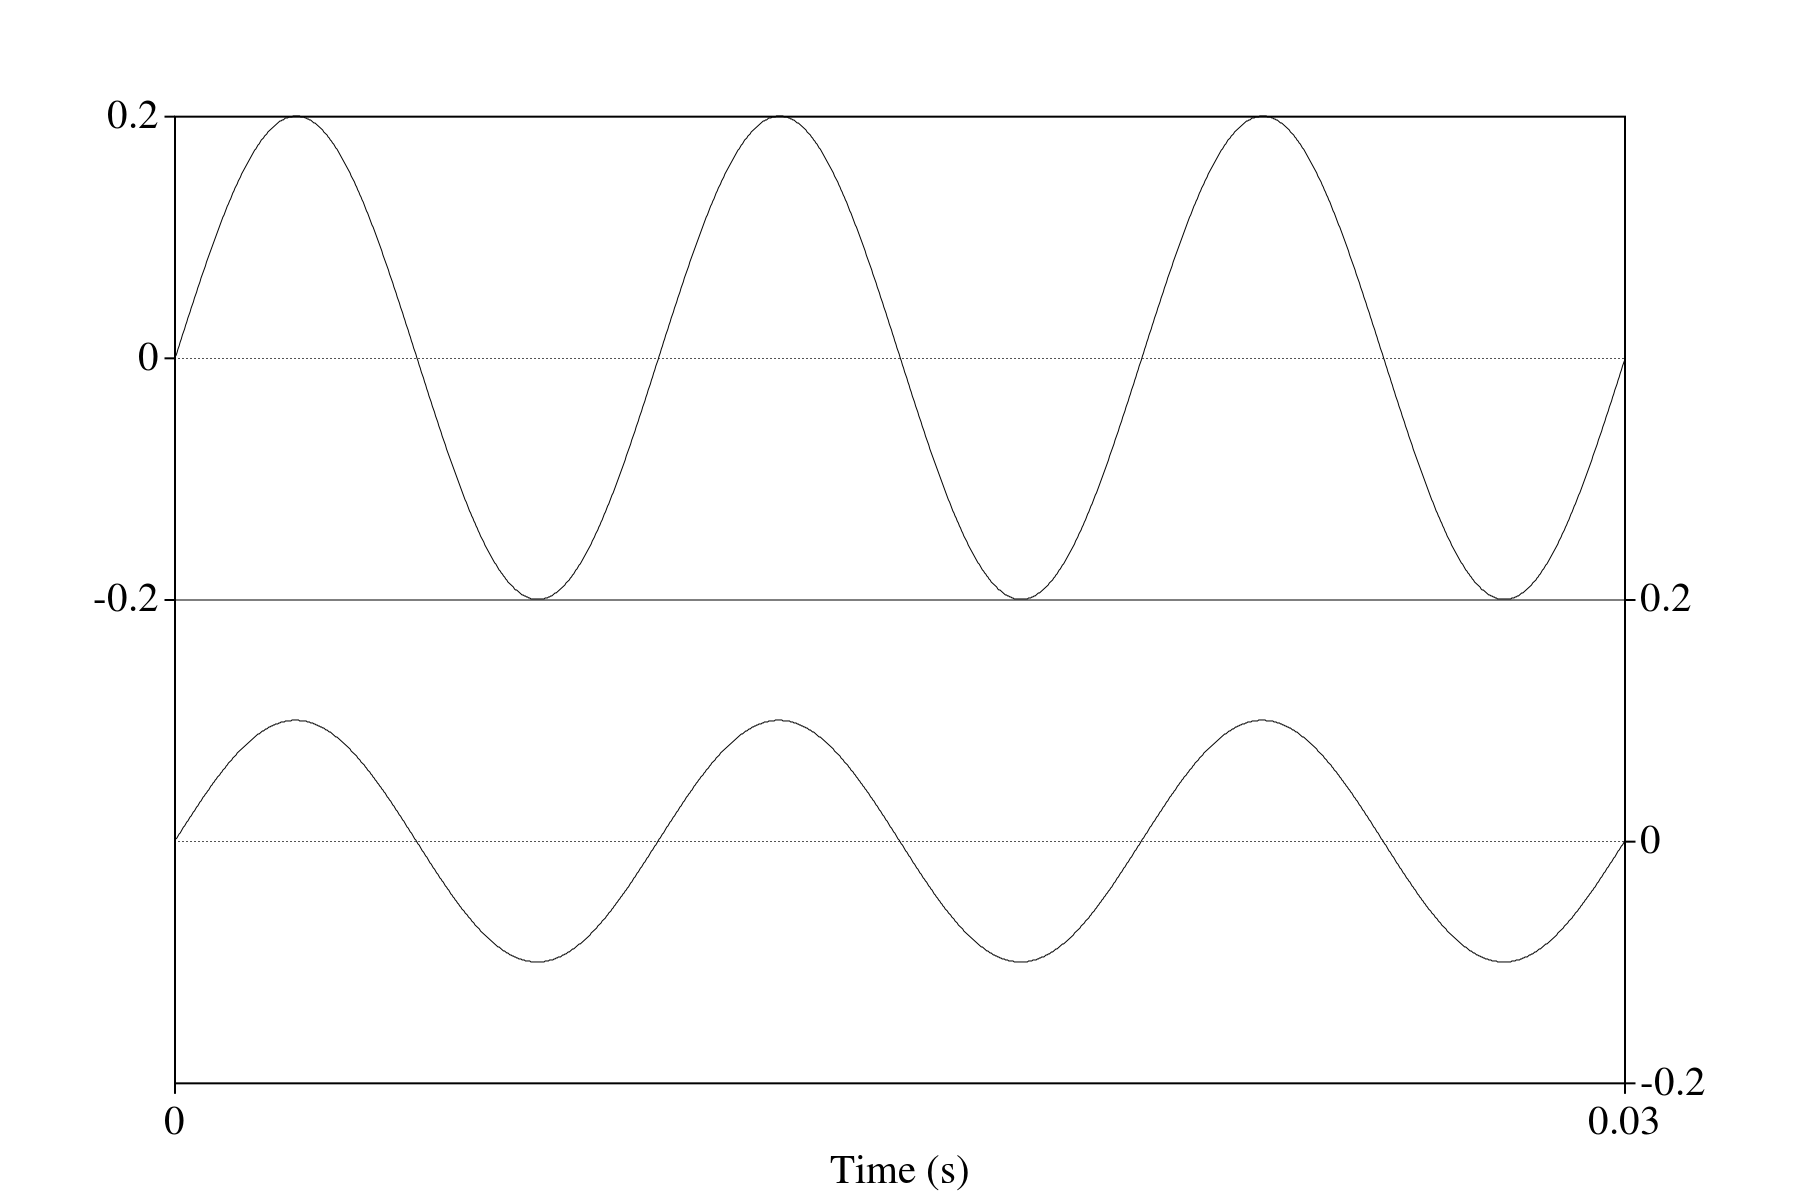
\includegraphics[width=\textwidth]{figure/basic-sound-amplitude.png}
  \caption{Two waveforms showing a difference in amplitude between the two signals.}
  \label{fig:basic-sound-amplitude}
\end{subfigure}
\qquad
\begin{subfigure}{0.5\textwidth}
  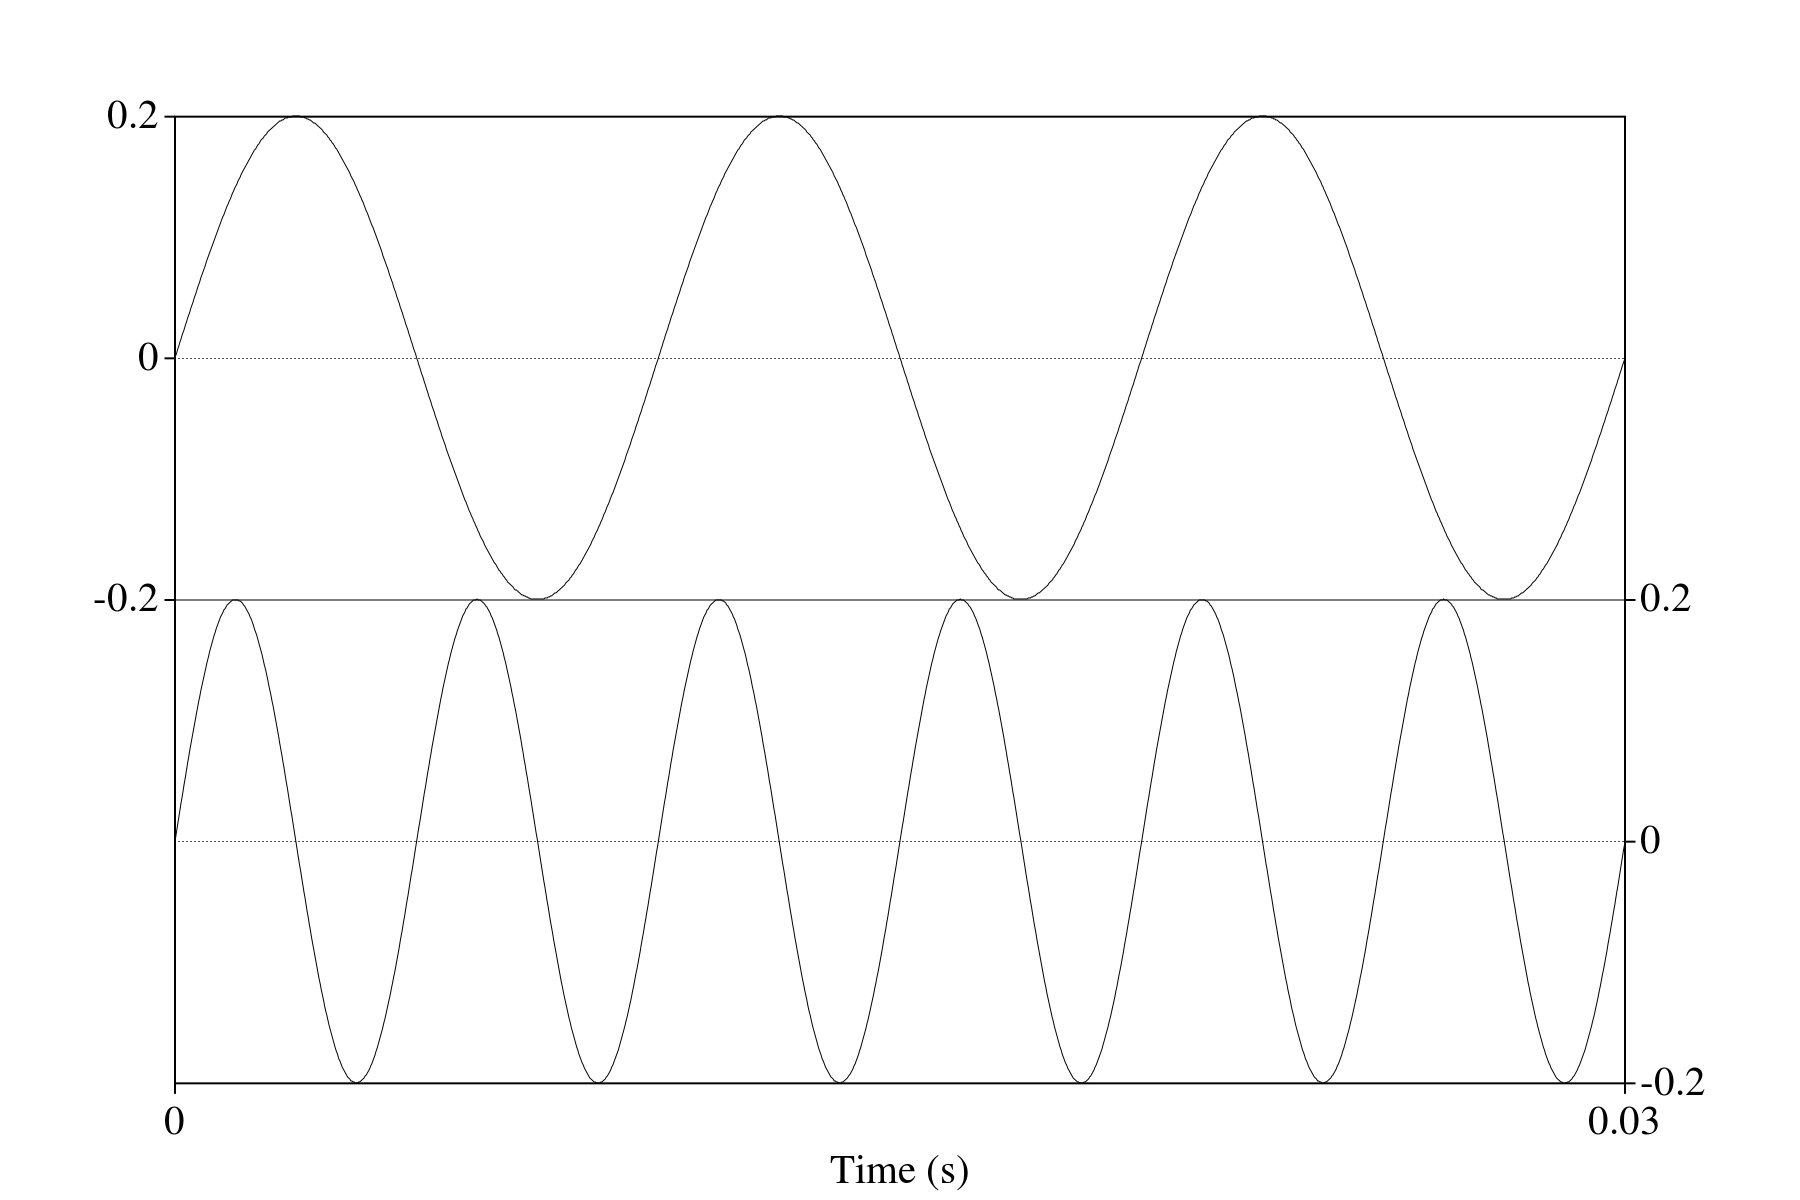
\includegraphics[width=\textwidth]{figure/basic-sound-frequency.png}
  \caption{Two waveforms showing a difference in frequency between the two signals.}
  \label{fig:basic-sound-frequency}
\end{subfigure}
%
\\[2ex]
\begin{center}
\begin{subfigure}{0.5\textwidth}
  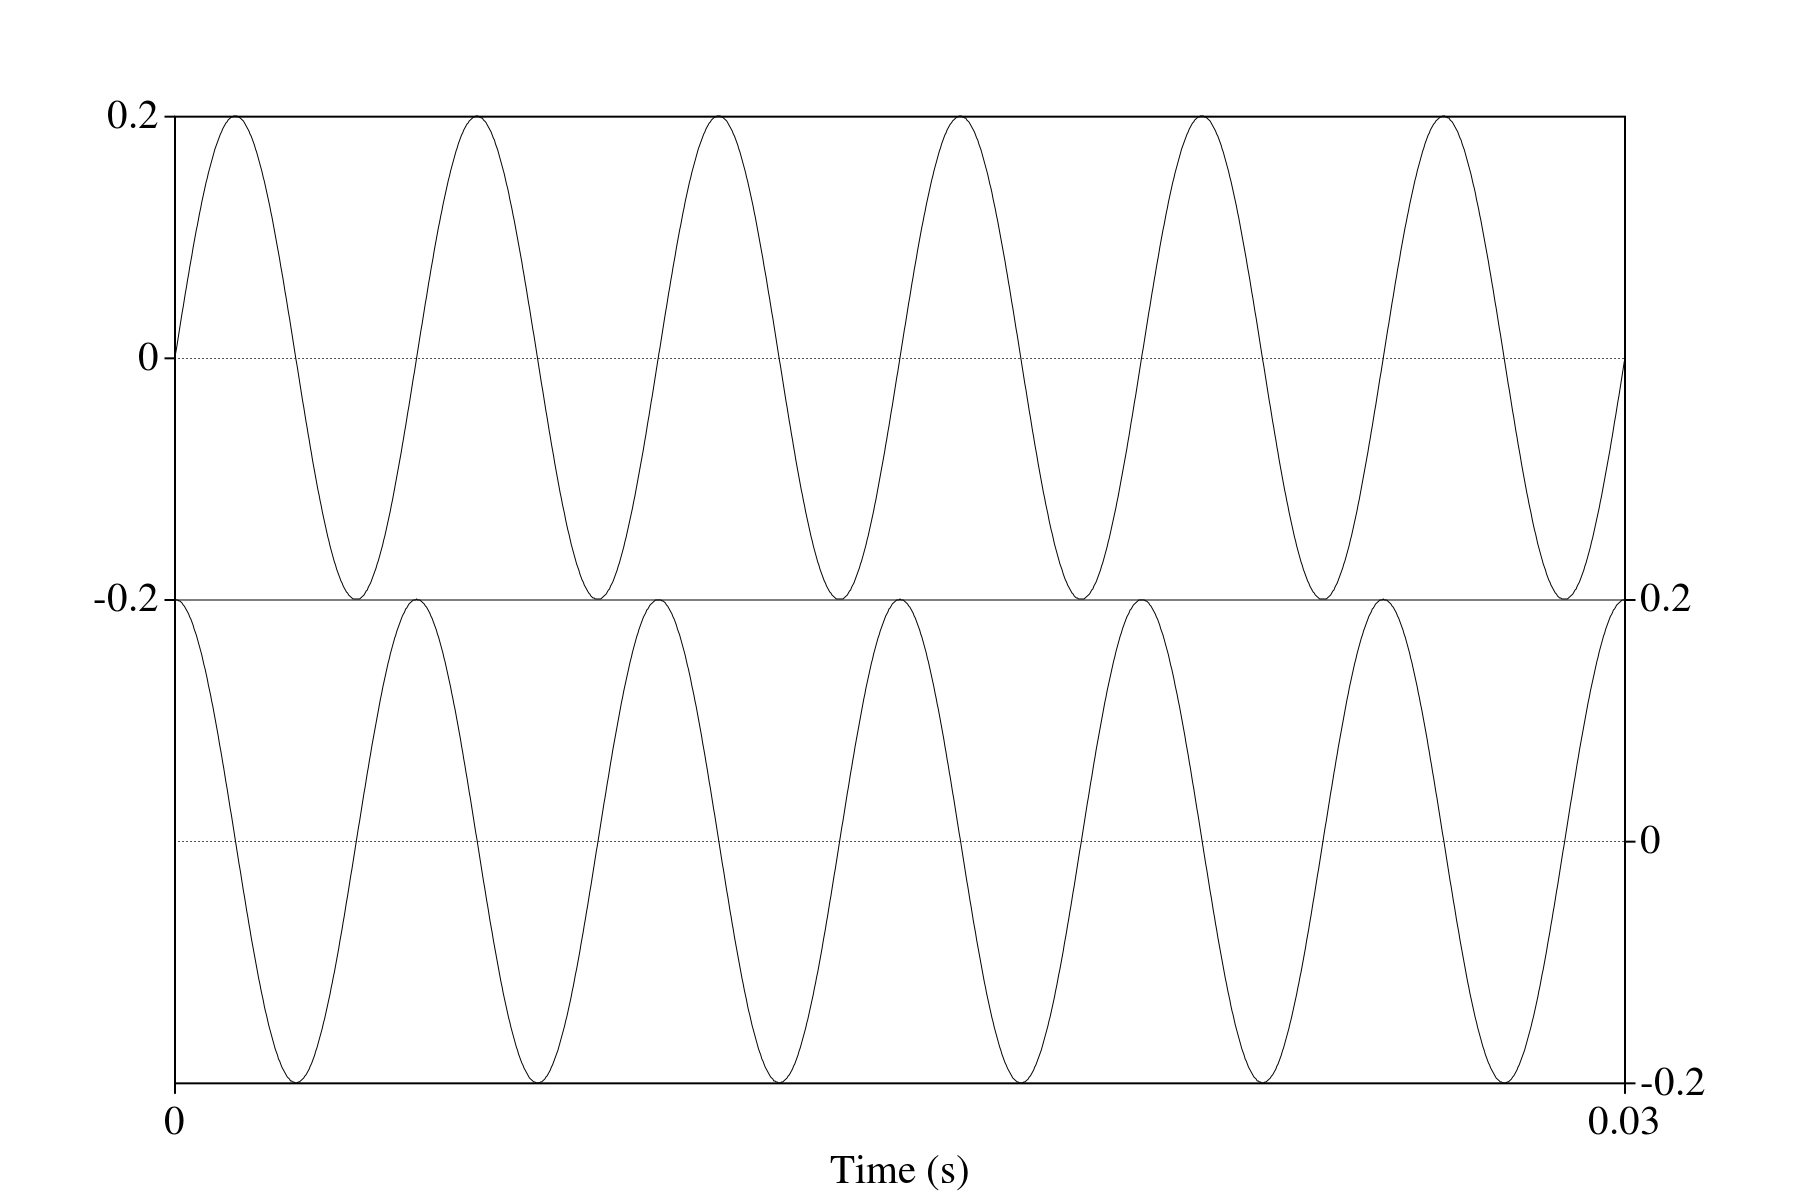
\includegraphics[width=\textwidth]{figure/basic-sound-phase.png}
  \caption{Two waveforms showing a difference in phase between the two signals.}
  \label{fig:basic-sound-phase}
\end{subfigure}
\end{center}
\caption{Waveforms demonstrating difference in amplitude, frequency, and phase.}
\label{fig:basic-sound-wave}
\end{figure}

This latter characteristic - phase, while important when dealing with interacting waves from multiple sources, is often not taken into in speech science due to both its complexity and the fact that phase does not encode any speech information.  The human auditory system primarily makes use of the other two characteristics of sound - amplitude and frequency.

\subsection{Overview of Anatomy and Physiology of the Peripheral Auditory System}

Prior to discussing the acoustic structure of speech, it is important to become familiar with the basic peripheral auditory system.  The peripheral auditory system is generally grouped into three primary categories, the outer ear, the middle ear, and the inner ear (cf. Figure \ref{fig:ear-anatomy}).  The outer ear includes the pinna, the ear canal tube, and the tympanic membrane (ie. the eardrum).  Air-transmitted sound vibrations, ie. pressure fluctuations, enter the ear canal through the opening at the pinna.  These then travel along the canal to vibrate the tympanic membrane, which passes the energy to the middle ear.  The middle ear includes the ossicles within the middle ear cavity.  The ossicles are a chain of three very small bones leading from the tympanic membrane to the cochlea. The external sound vibrations hit the tympanic membrane, are passed along the ossicle chain, which then sends these vibrations to the inner ear.

\begin{figure}[h]
\centering
  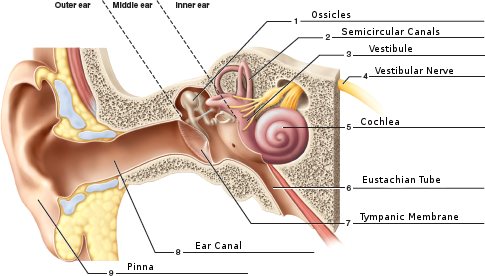
\includegraphics{figure/ear_anatomy.png}
  \caption{A diagram of the peripheral auditory system, including the outer ear, middle ear, and inner ear, up to the auditory nerve. (Image from \cite{martin:12})}
  \label{fig:ear-anatomy}
\end{figure}

The inner ear is composed of the cochlea, the semicircular canals (and vestibule), and the auditory and vestibular nerves.  The semicircular canals, vestibule, and vestibular nerve don't play a part in audition (their primary function regards balance sensitivity).  The cochlea, a hard `shell' filled with fluid receives the vibrations passed along through the middle ear ossicles.\footnote{The peripheral auditory system uses gas, solid, and liquid media to transmit acoustic vibrations.}  The vibrations are passed into the fluid cochlea and travel along the length of the cochlea, transmitting acoustic energy to cells that are able to detect the amplitude of the vibrations.  Depending on the location of a cell along the length of the cochlea, it will pick up a different frequency of sound.  The auditory nerve carries electrical impulses from these cells into the auditory cortex of the brain. 

Of interest to this present study is the relatively simple outer ear.  Typically, as described above, vibrations from the air will enter the ear canal through the opening at the pinna. Frequently, these vibrations take the form of human speech.

%However, vibrations from one's own speech are also transmitted via the bone, cartilage, and tissue of the head.  Regardless of source, sound vibrations entering into the ear canal will be altered by the shape of the ear canal, described more below.


\subsection{Acoustic Structure of Human Speech}

The structure of human speech draws from a collection of individual sounds (phonemes) that are strung together, encoding words, sentences, and more abstractly, meaning.  Each human language uses a subset of all possible phonemes.  Each phoneme is either considered `voiced' or `unvoiced'.  The acoustic properties of sounds in these two categories differ greatly.

Voiced speech is composed of narrow bands of acoustic energy, called harmonics, located along a frequency spectrum (cf. fig \ref{fig:spctrm5k}).  In this sense, speech is considered a `complex' sound, because it is composed of multiple, simultaneous frequencies.
%
\begin{wrapfigure}{l}{0.5\textwidth}
\centering
  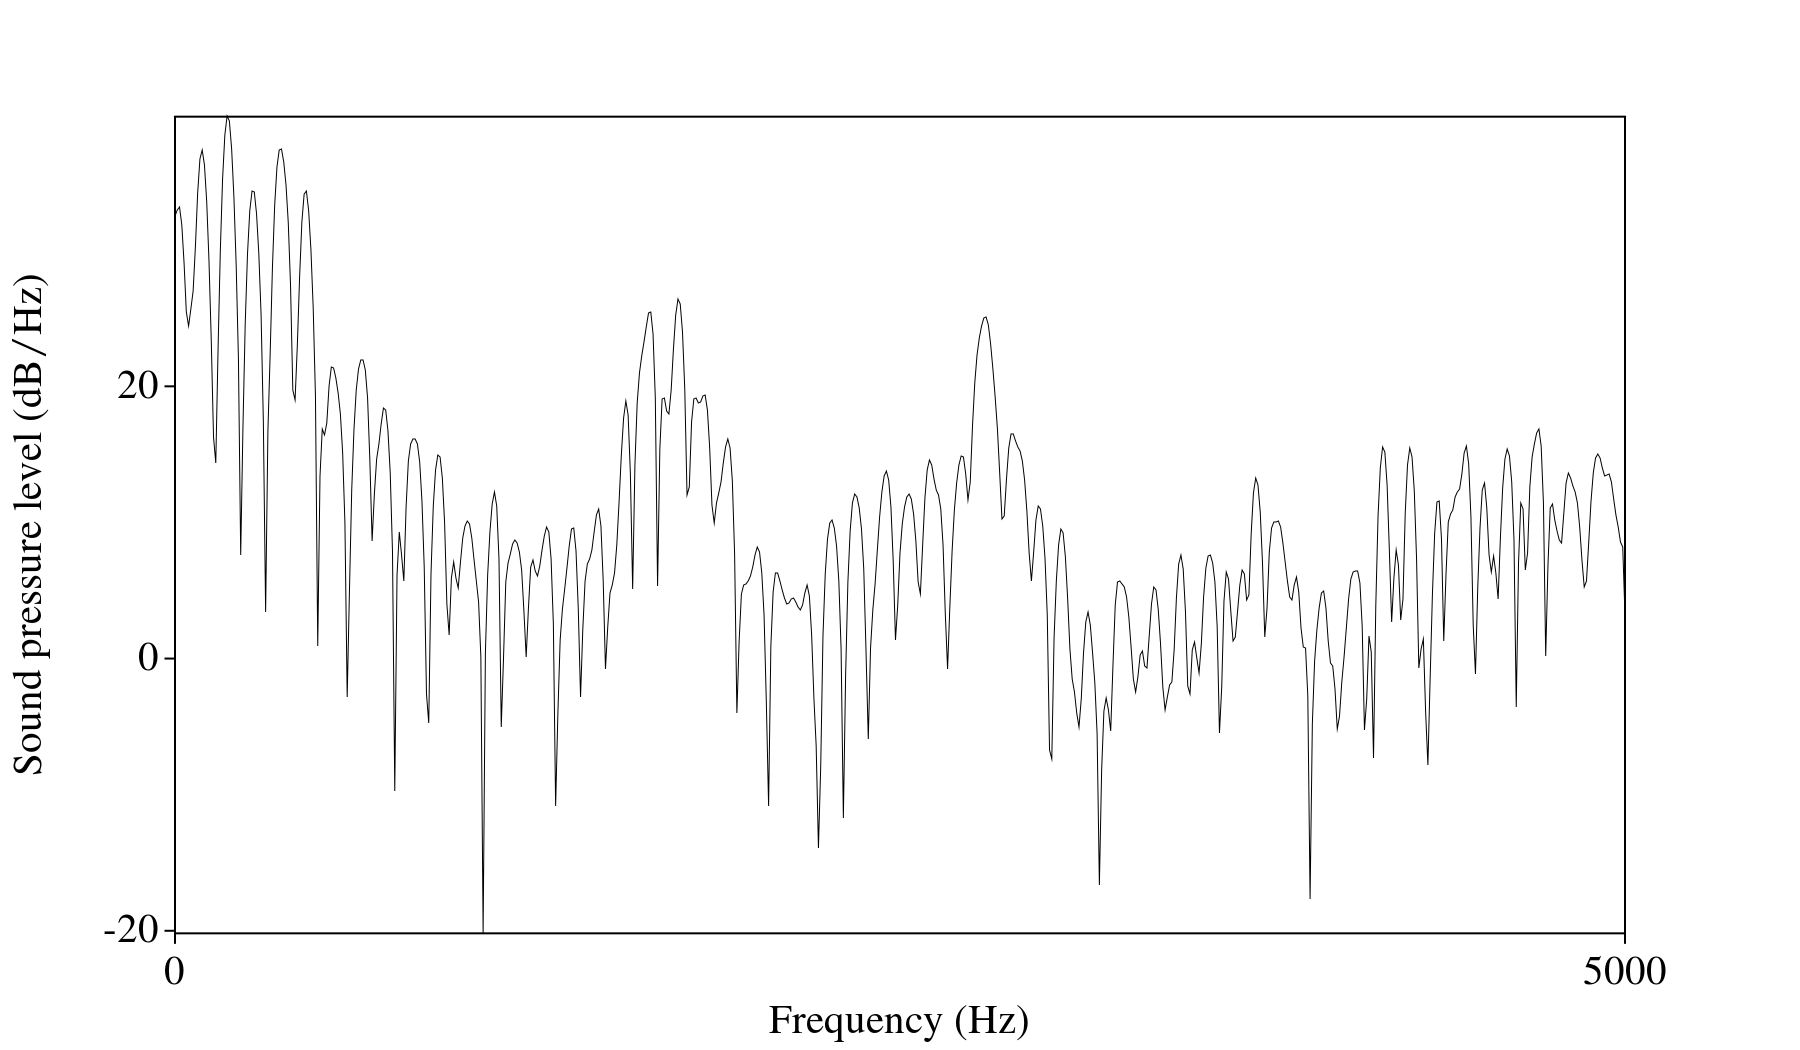
\includegraphics[width=0.5\textwidth]{figure/spctrm5k.png}
  \caption{Spectrum of the middle of an /I/ vowel.  Each `spike' is a separate narrow band of frequency, called a harmonic.}
  \label{fig:spctrm5k}
\end{wrapfigure}
%
Certain harmonics will be dampened by the vocal tract, leaving others relatively unfiltered.  A group of neighboring harmonics containing more energy than other harmonics are called formants.  The location, shape, and transition over time of these formants (among other more minor features) are what encodes speech information for voiced sounds.  This can be easily visualized in a spectrogram (cf. Fig. \ref{fig:spctgrm_citizen}).

\begin{figure}[h!]
\begin{subfigure}{0.95\textwidth}
  \centering
  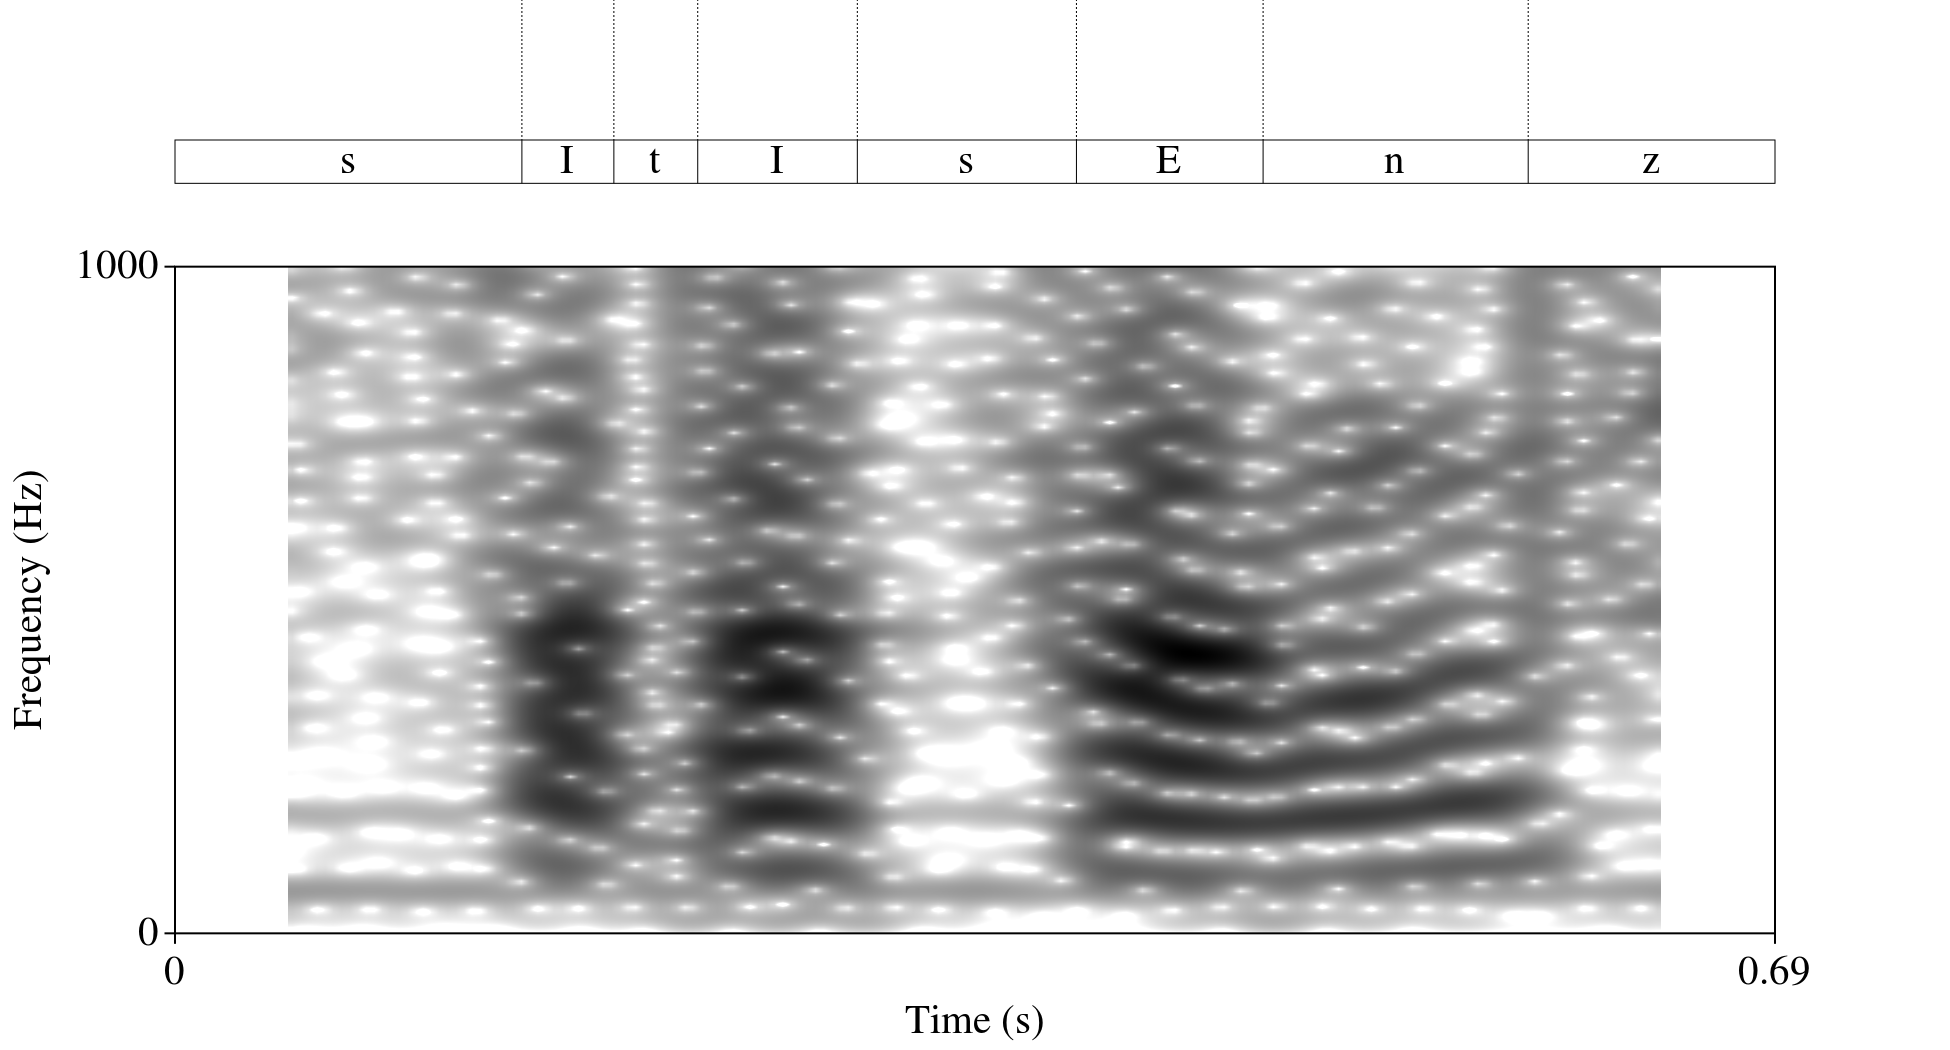
\includegraphics[width=0.95\textwidth]{figure/spctgrm1k.png}
  \caption{Zoomed to the 0-1kHz range for better visualization of harmonics.}
  \label{fig:spctgrm_citizen_1k}
\end{subfigure}%
\hfill
\begin{subfigure}{0.95\textwidth}
  \centering
  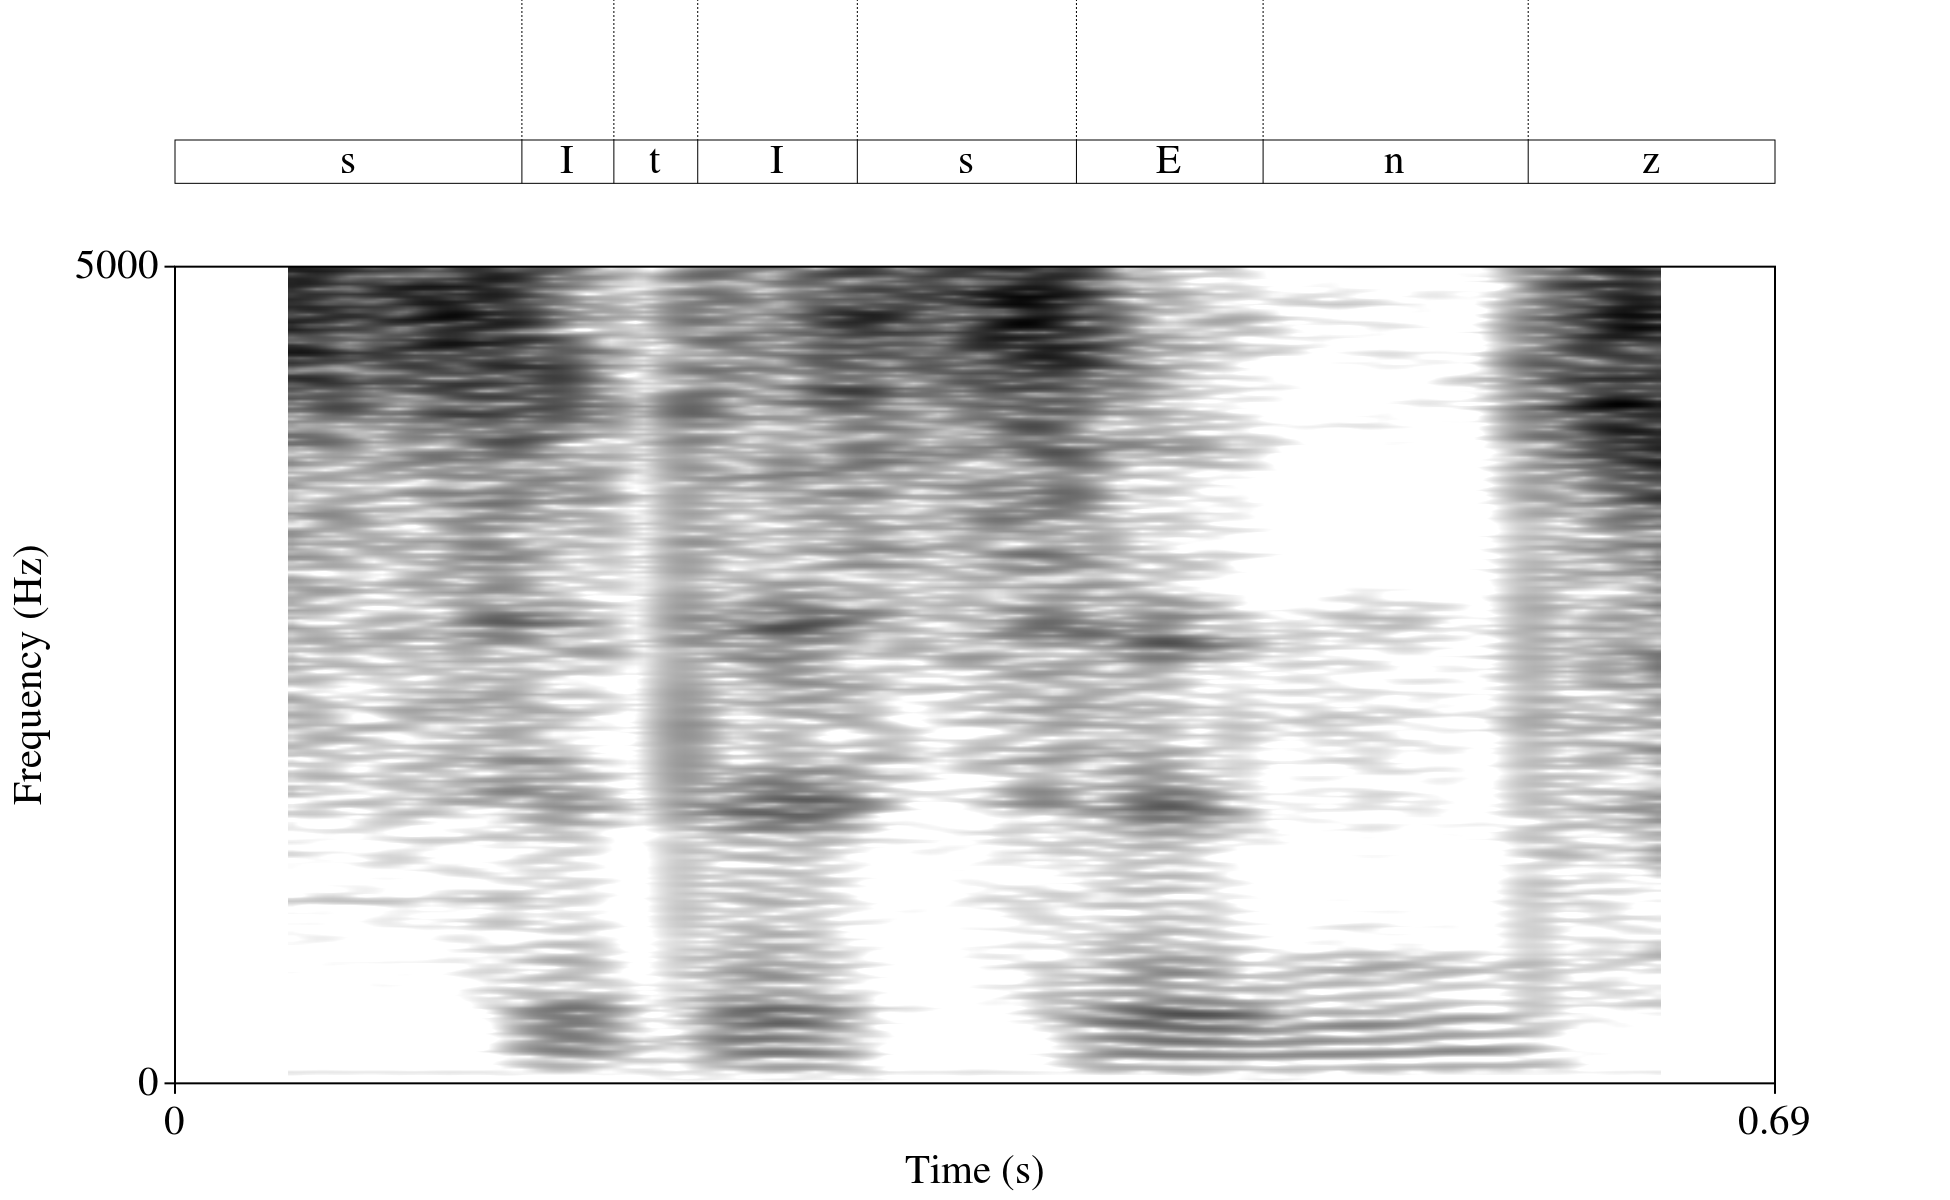
\includegraphics[width=0.95\textwidth]{figure/spctgrm5k.png}
  \caption{Zoomed to a more standard 0-5kHz range.}
  \label{fig:spctgrm_citizen_5k}
\end{subfigure}
\caption{Spectrogram of the word ``citizens'' with phonetic transcription above.  Frequency is on the y-axis, time is on the x-axis, and amplitude is shown in grayscale on the graph; the darker an area of the graph, the greater the amplitude.}
\label{fig:spctgrm_citizen}
\end{figure}

For unvoiced speech, the information used to recognize and categorize the speech sound is likely found in either the turbulent frication generally centered in higher frequencies (cf. Fig. \ref{fig:spctgrm_s}, although some of the information can be found in lower frequencies), or found in the voiced information in the transitions into and out of the sound (\cite{willi:17}).
%
\begin{wrapfigure}{l}{0.5\textwidth}
\centering
  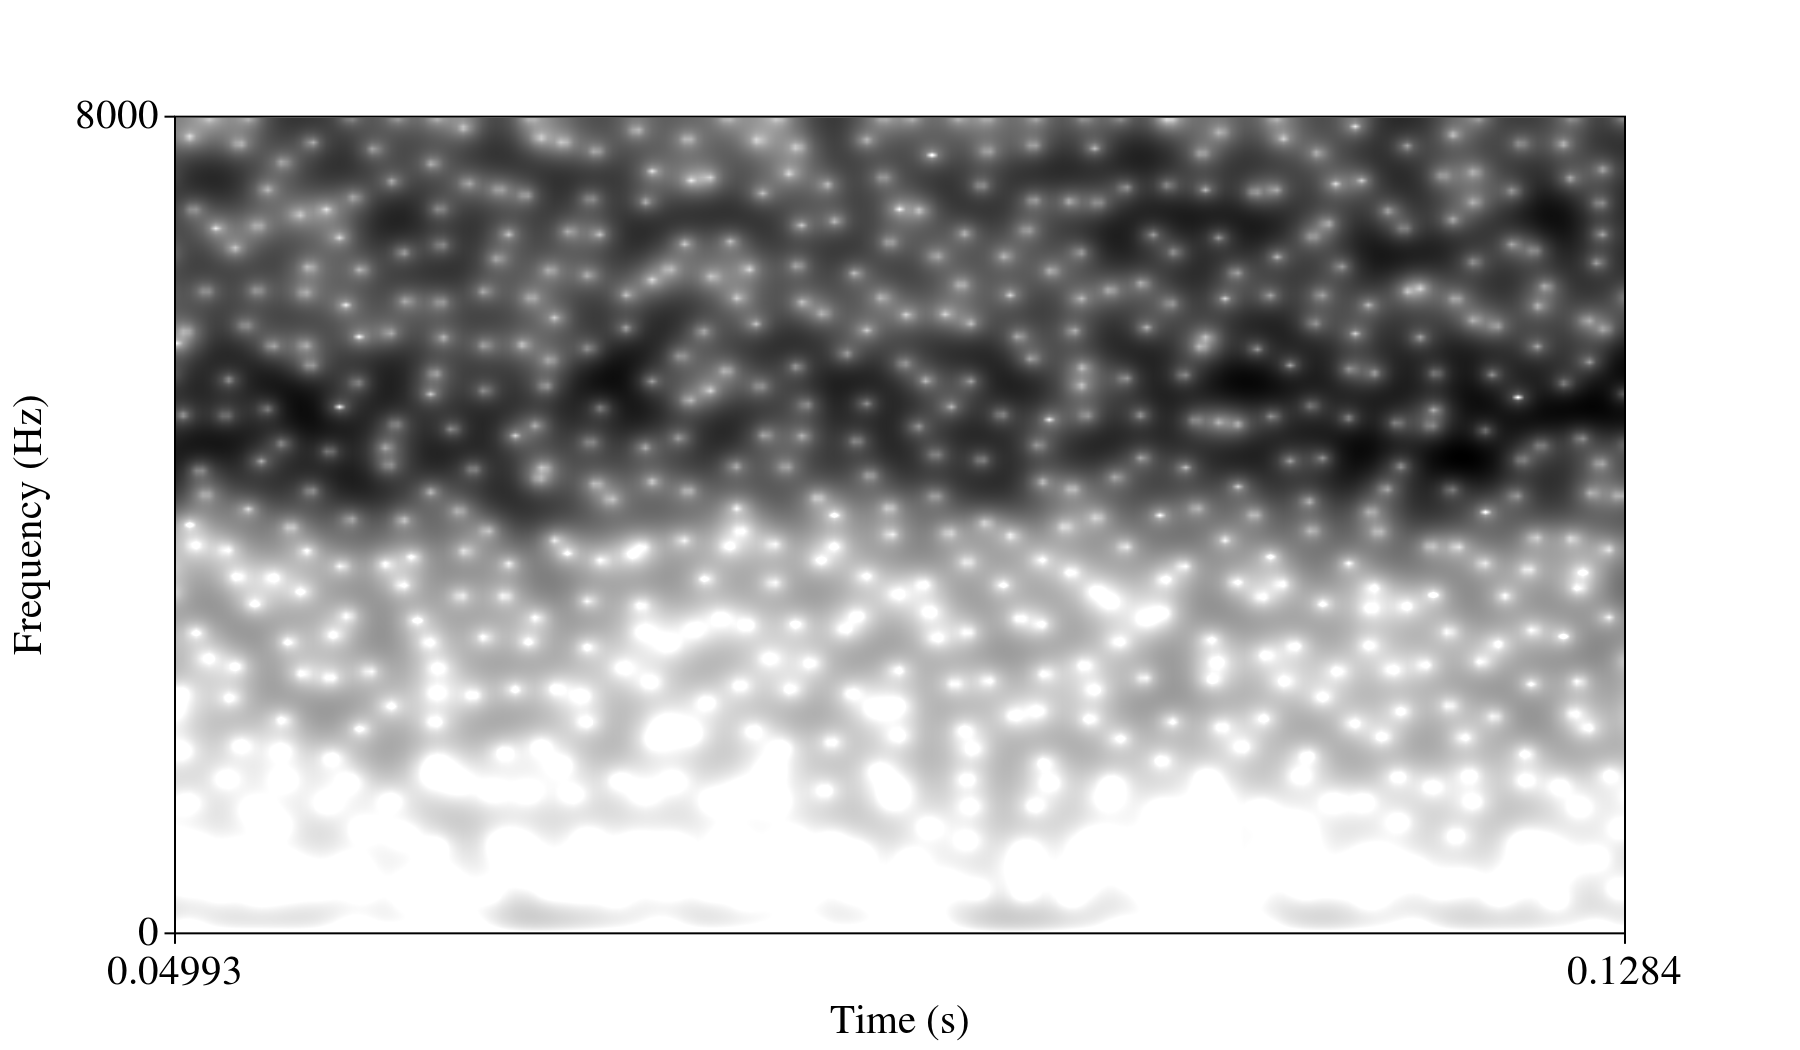
\includegraphics[width=0.5\textwidth]{figure/spctgrm_s.png}
  \caption{Spectrum of the initial /s/ in ``citizen''. Zoomed to range of 0-8kHz for visualization of high frequency energy.}
  \label{fig:spctgrm_s}
\end{wrapfigure}

The human auditory system has the remarkable ability to (a) identify these sounds, which often only last from tens to a few hundreds of milliseconds in duration, (b) partition the stream of sounds into their respective words, and (c) string the words together into a sentence and pull meaning from it - all in real time.  Nevertheless there are occasionally recognition errors, which can occur anywhere along this auditory chain.  The `lowest' level in this chain that errors occur is the recognition and identification of sounds.  There are a host of reasons why this might occur, yet this report will focus on one of them - additive noise interfering with the speech signal.

\subsection{Acoustics of Multiple Signals}

As previously mentioned, we as humans use the amplitude and frequency of pressure fluctuations to perceive sound. When sound travels through a medium from source \textit{A}, there is nothing that prevents these pressure fluctuations of source \textit{A} from acoustically mixing with the pressure fluctuations originating from source \textit{B}.  For example, in Figure \ref{fig:sound-wave-addition} source \textit{A} produces a simple wave with a frequency of 100 Hz.  Source \textit{B} produces a simple wave with a frequency of 200 Hz.  If the waves from the two sources reach each other and overlap, a single wave results that looks like that in Figure \ref{fig:sound-wave-addition-combined}.  This sound wave now has two components - a tone at 100 Hz and a tone at 200 Hz.

\begin{figure}[h!]
\begin{subfigure}{0.5\textwidth}
  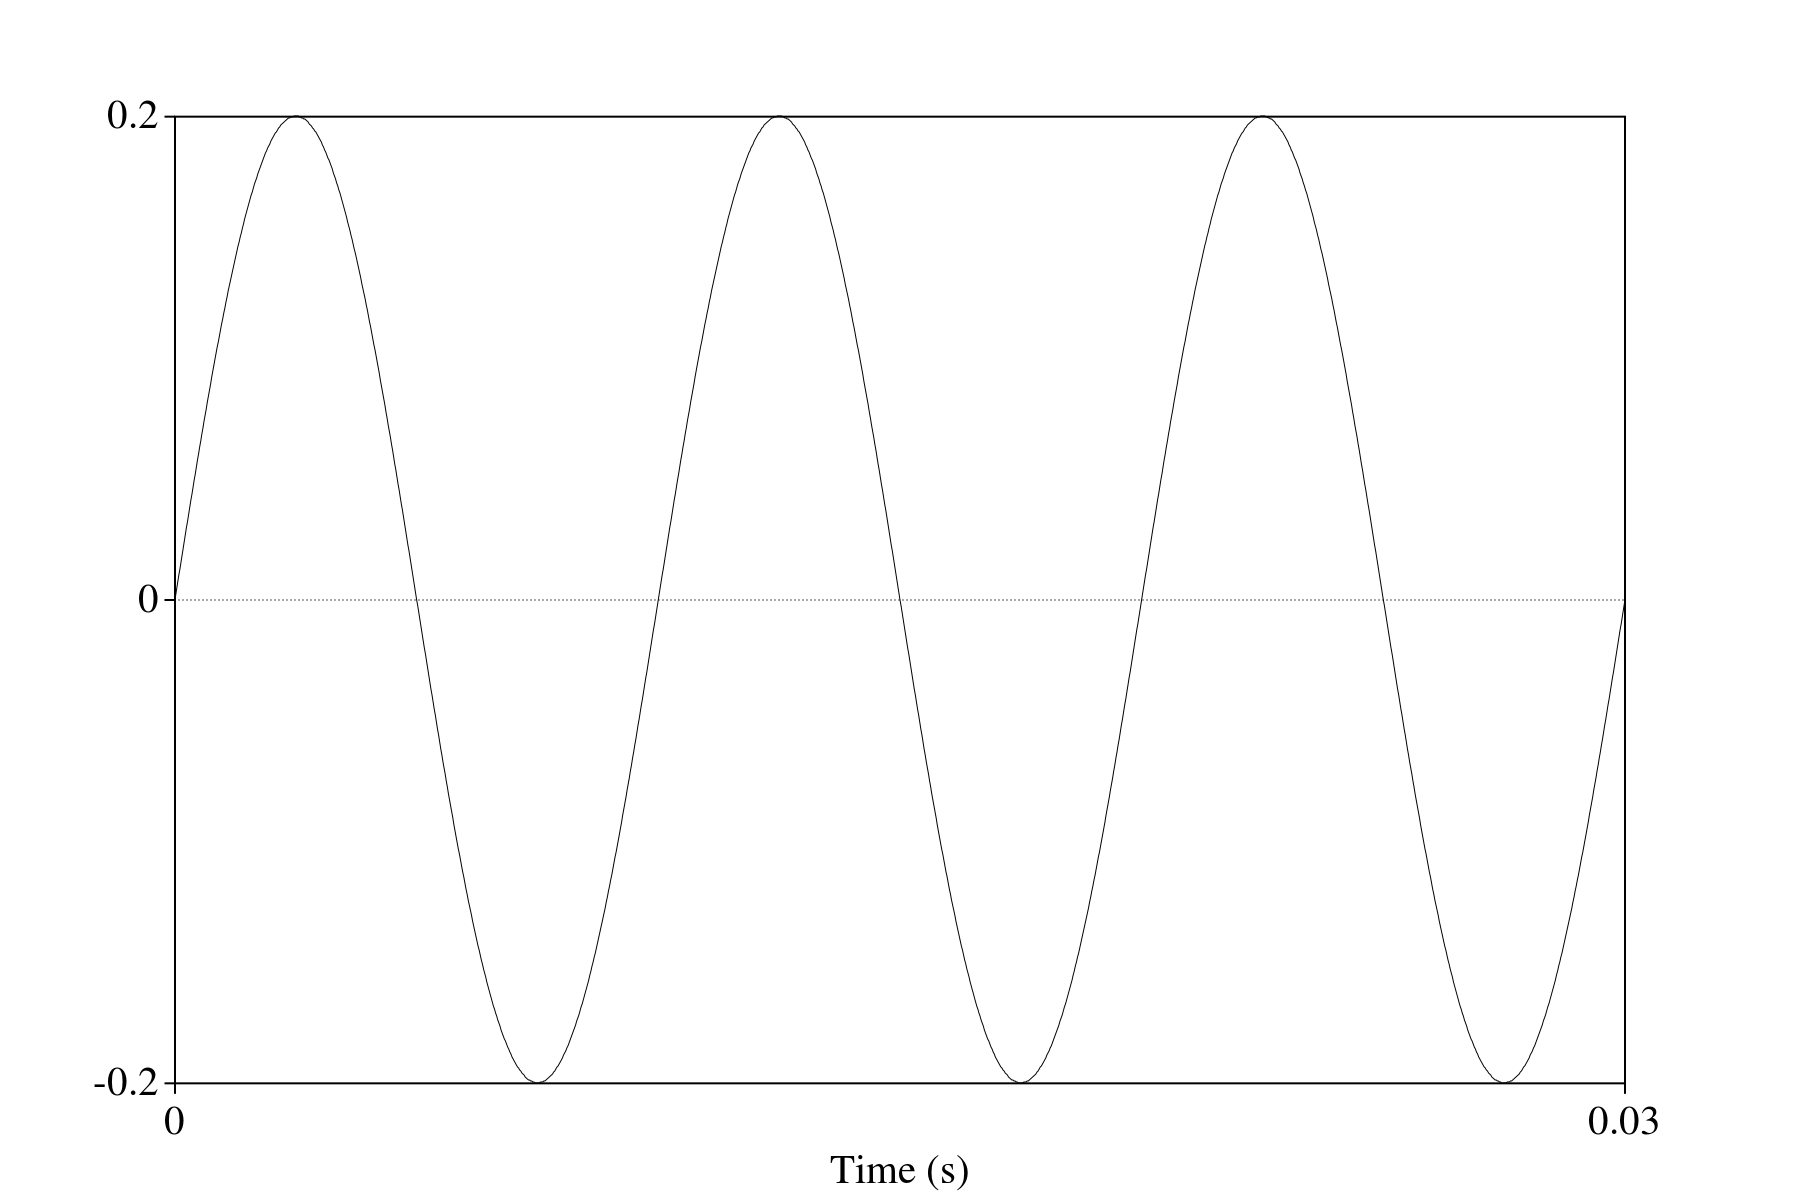
\includegraphics[width=\textwidth]{figure/basic-sound-wave.png}
  \caption{A basic sound wave from source \textit{A} at a frequency of 100 Hz.}
  \label{fig:sound-wave-A}
\end{subfigure}
\qquad
\begin{subfigure}{0.5\textwidth}
  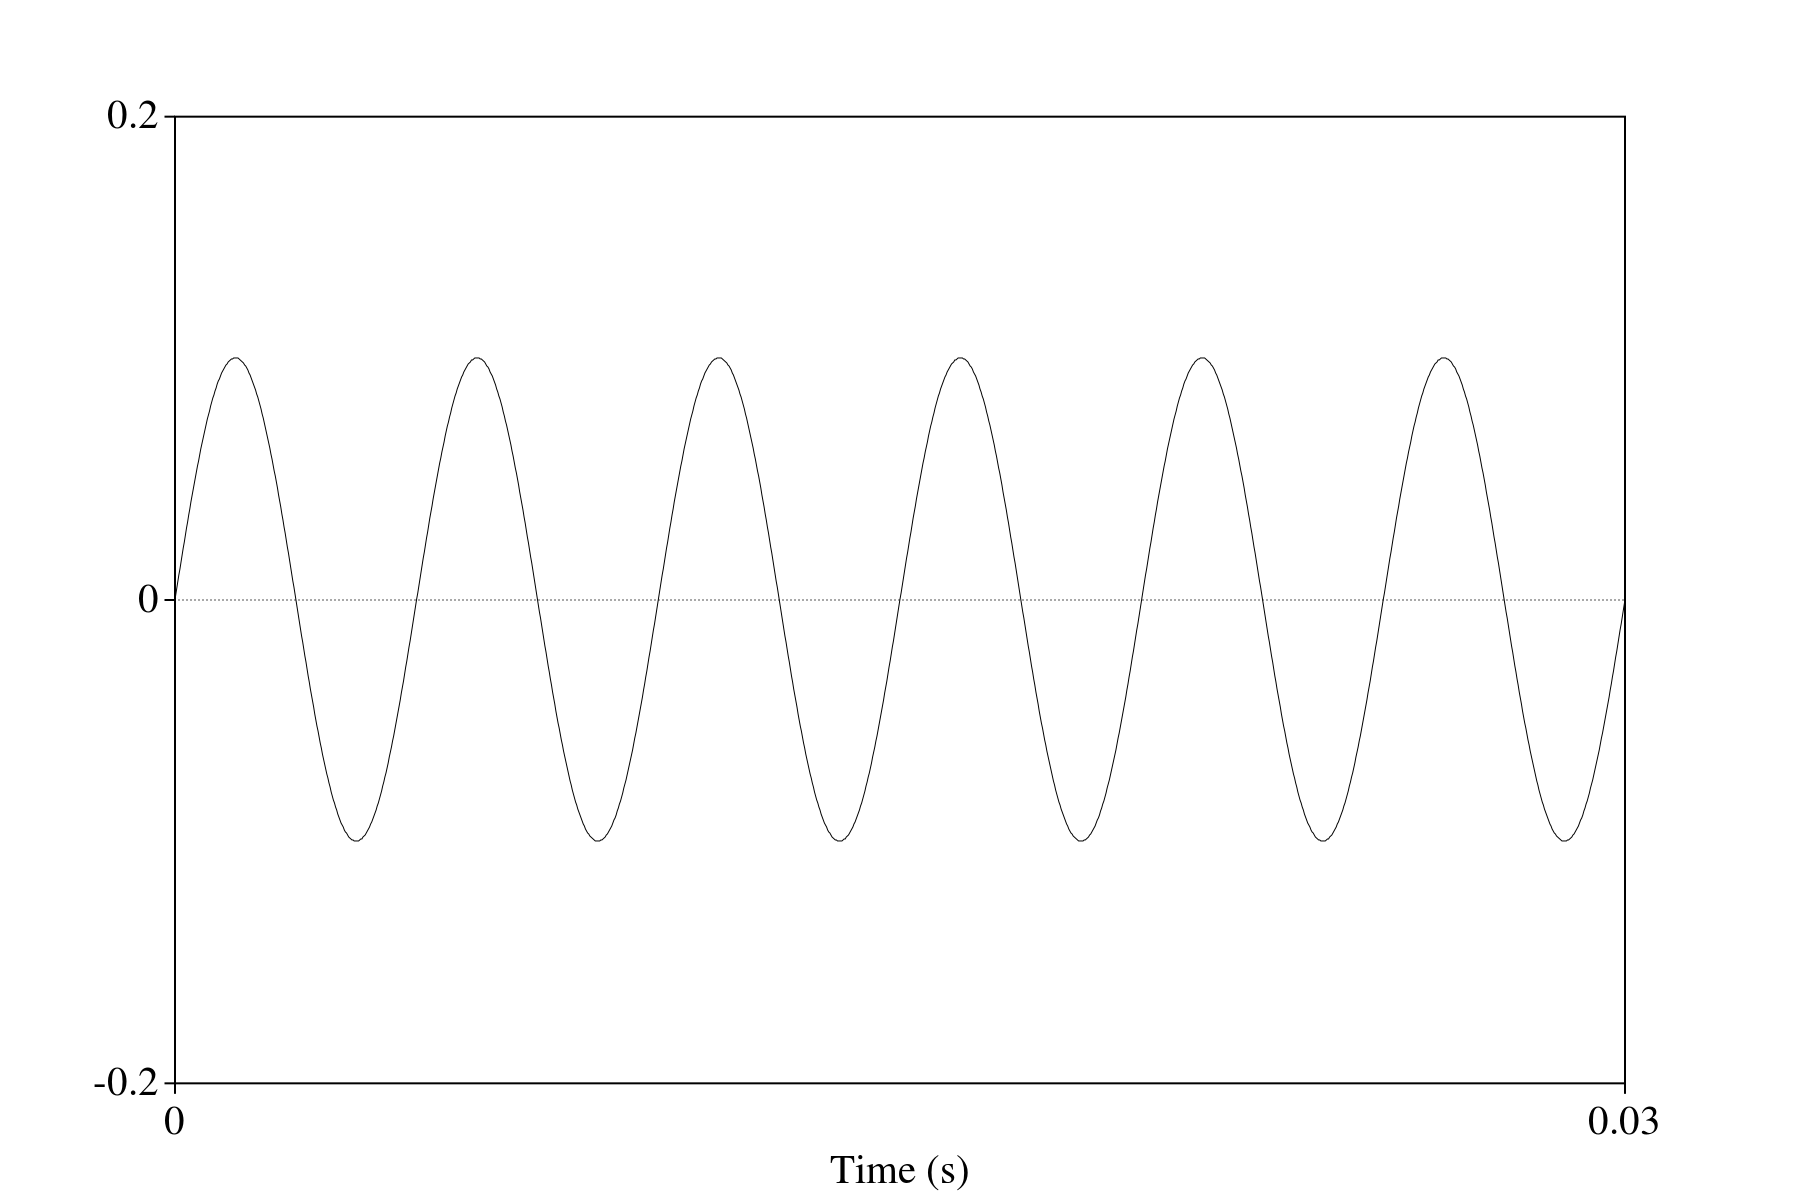
\includegraphics[width=\textwidth]{figure/sound-wave-addition-200hz.png}
  \caption{A basic sound wave from source \textit{B} at a frequency of 200 Hz, with half the amplitude of the simple sound wave from source \textit{A}.}
  \label{fig:sound-wave-B}
\end{subfigure}
%
\\[2ex]
\begin{center}
\begin{subfigure}{0.5\textwidth}
  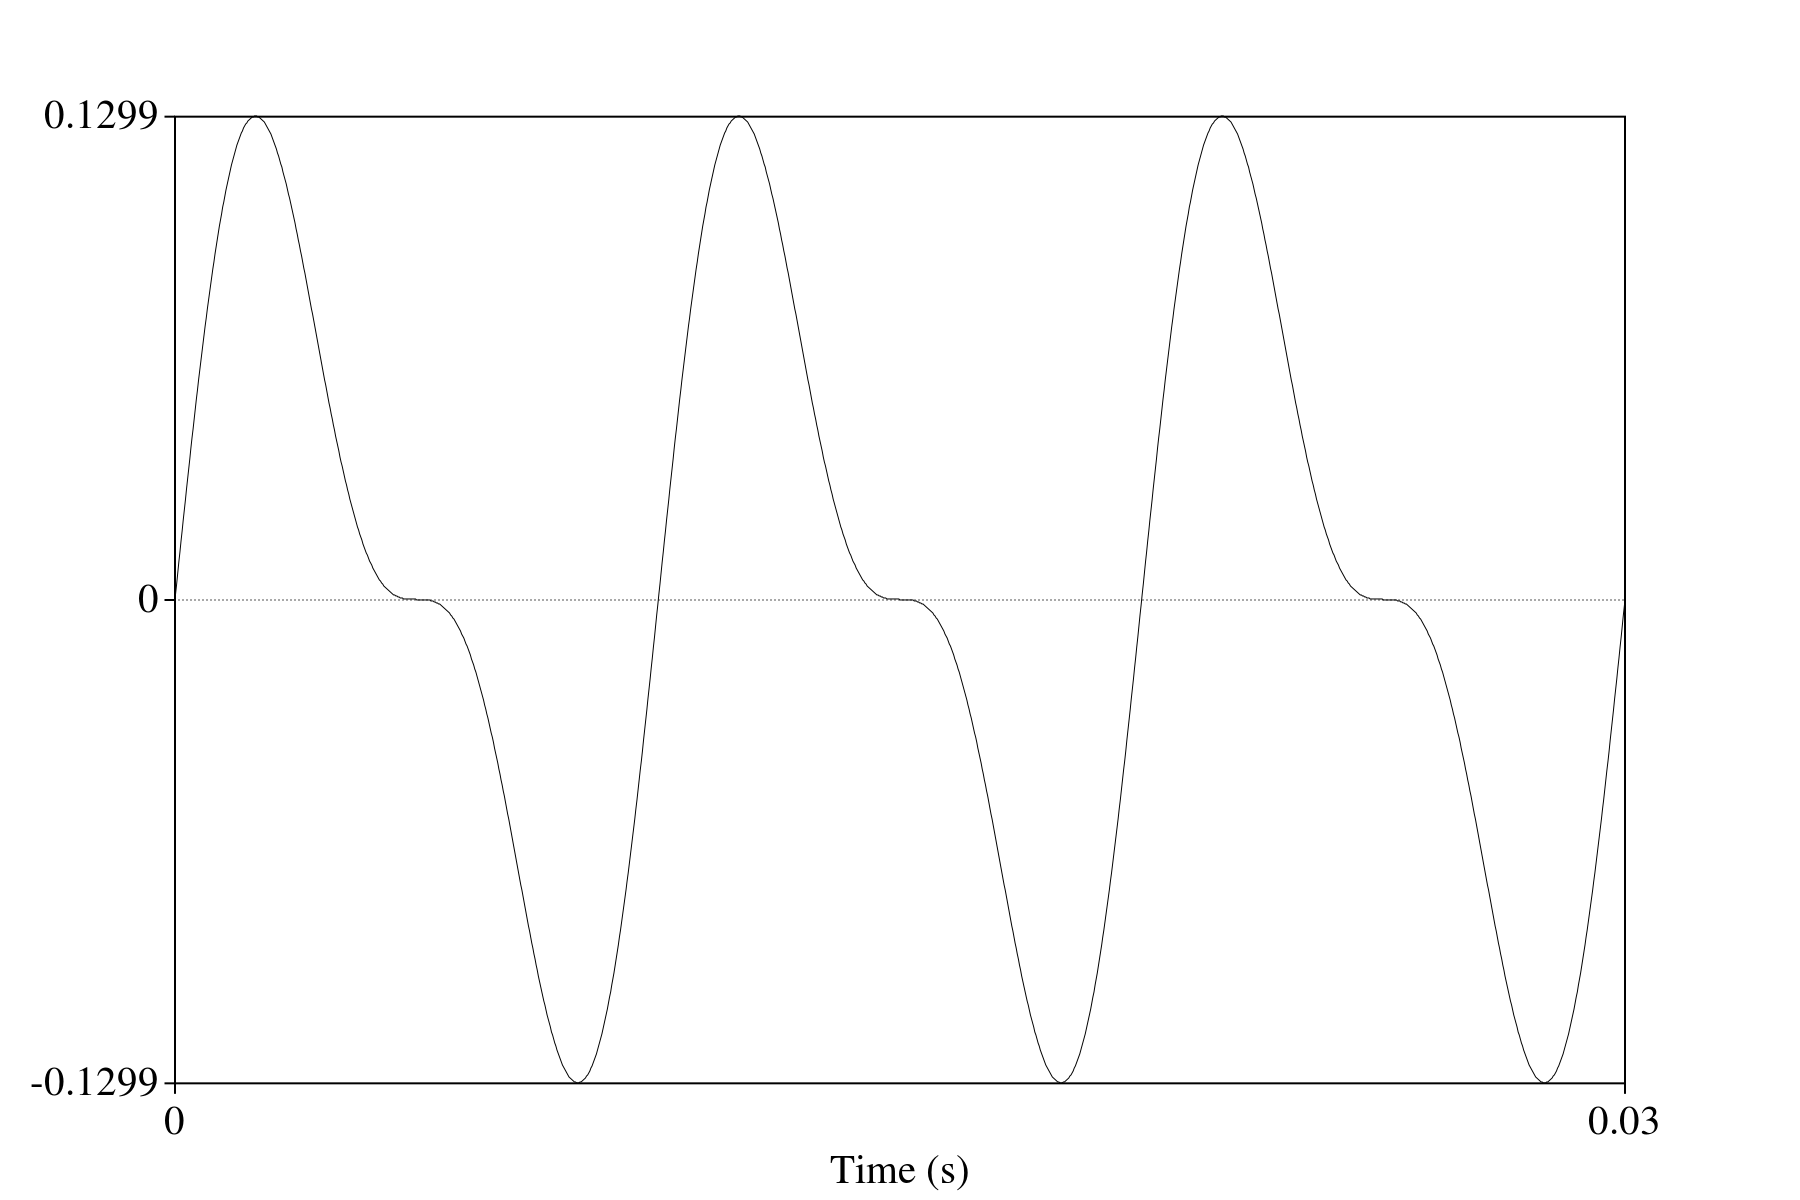
\includegraphics[width=\textwidth]{figure/sound-wave-addition-combined.png}
  \caption{The resulting complex wave from the combination of the wave from source \textit{A} and source \textit{B}.}
  \label{fig:sound-wave-addition-combined}
\end{subfigure}
\end{center}
\caption{Demonstration of the combination of two waves of different frequency and amplitude.}
\label{fig:sound-wave-addition}
\end{figure}

As previously mentioned, phase does not play a significant role in human audition, but can affect a wave resulting from the addition of multiple sound sources.  Say that source \textit{B} produces instead a wave the same frequency and amplitude as the wave from source \textit{A}, but they are completely `out of phase', ie. the pressure value of the waves at any given time is in direct opposition (cf. Figure \ref{fig:wave-out-of-phase}).  If these waves are combined, it results in a complete elimination of sound (cf. Fig. \ref{fig:wave-out-of-phase-added}).

\begin{figure}[h!]
\begin{subfigure}{0.5\textwidth}
  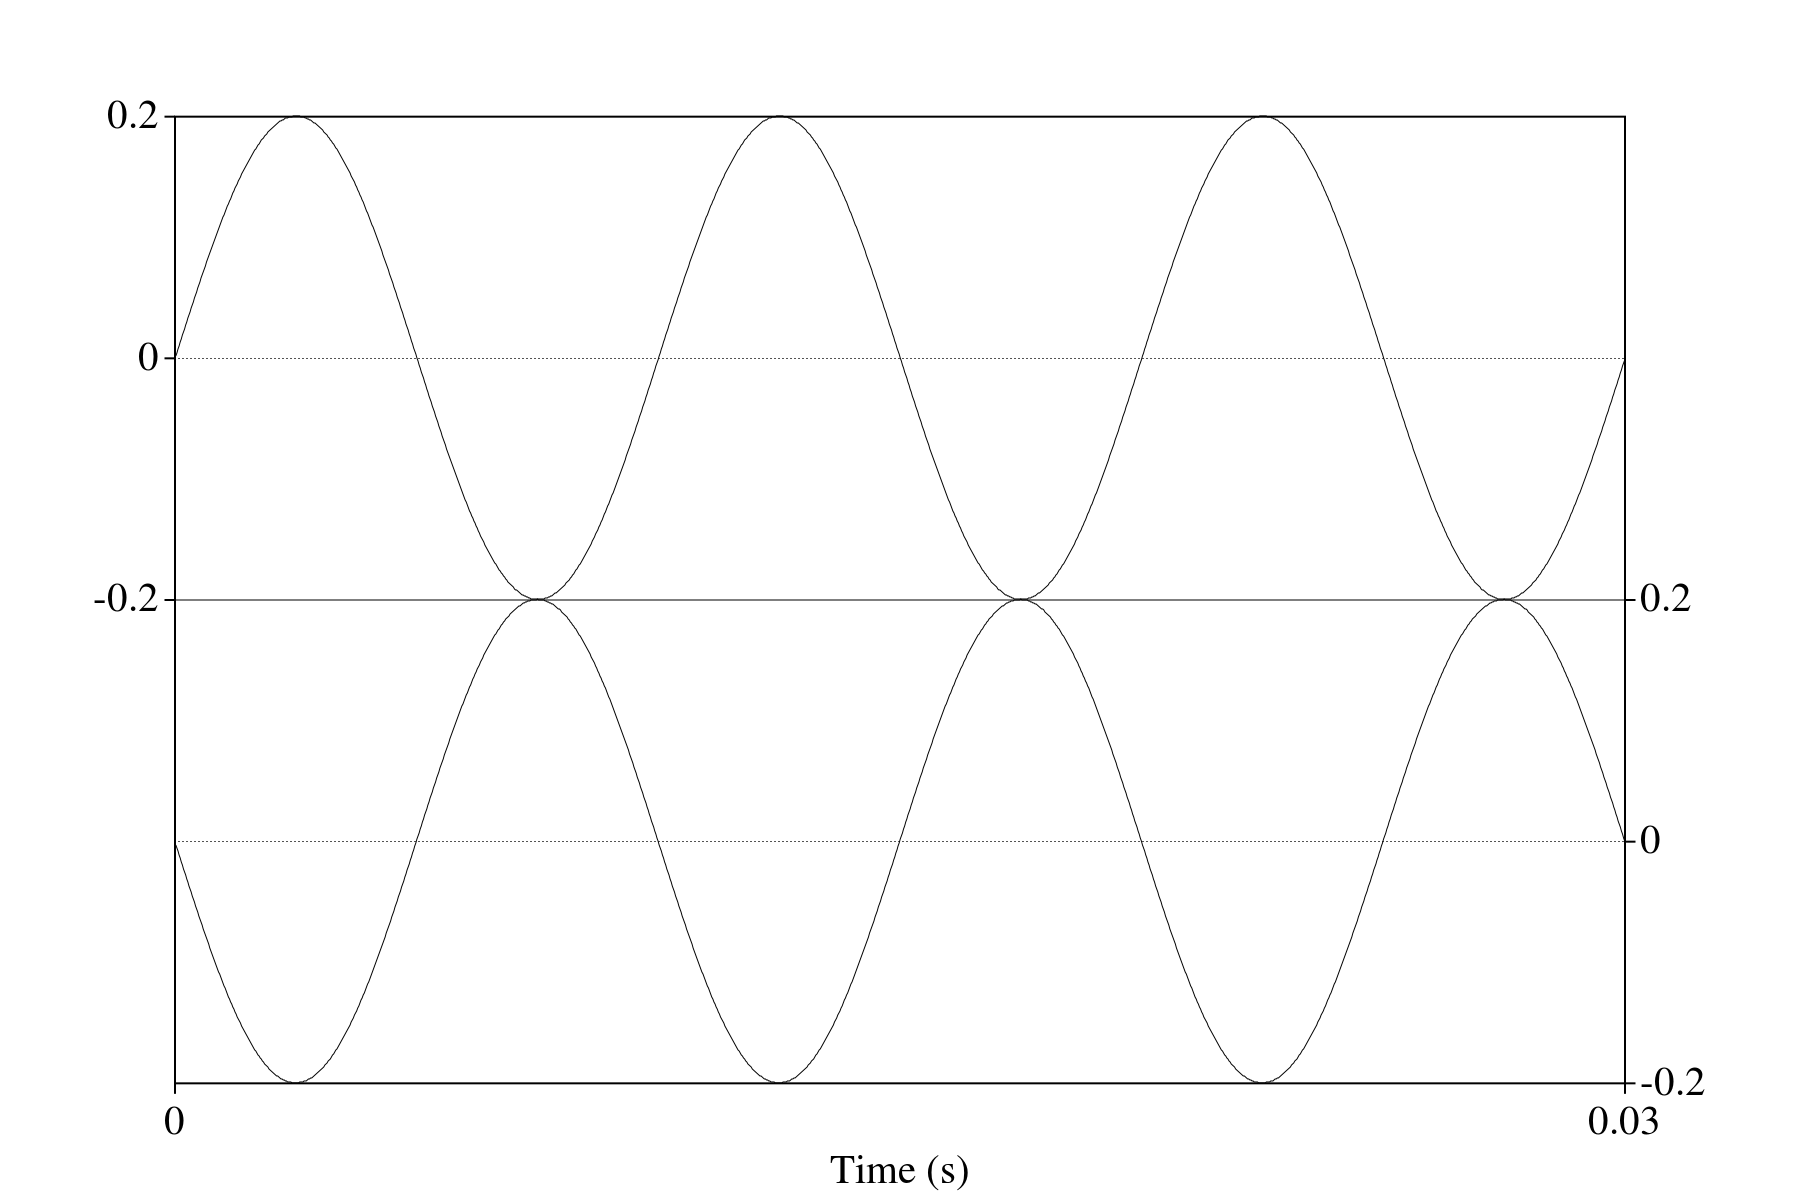
\includegraphics[width=\textwidth]{figure/wave-out-of-phase.png}
  \caption{Two sound waves with frequency of 100 Hz and the same amplitude, completely out of phase.}
  \label{fig:wave-out-of-phase}
\end{subfigure}
\qquad
\begin{subfigure}{0.5\textwidth}
  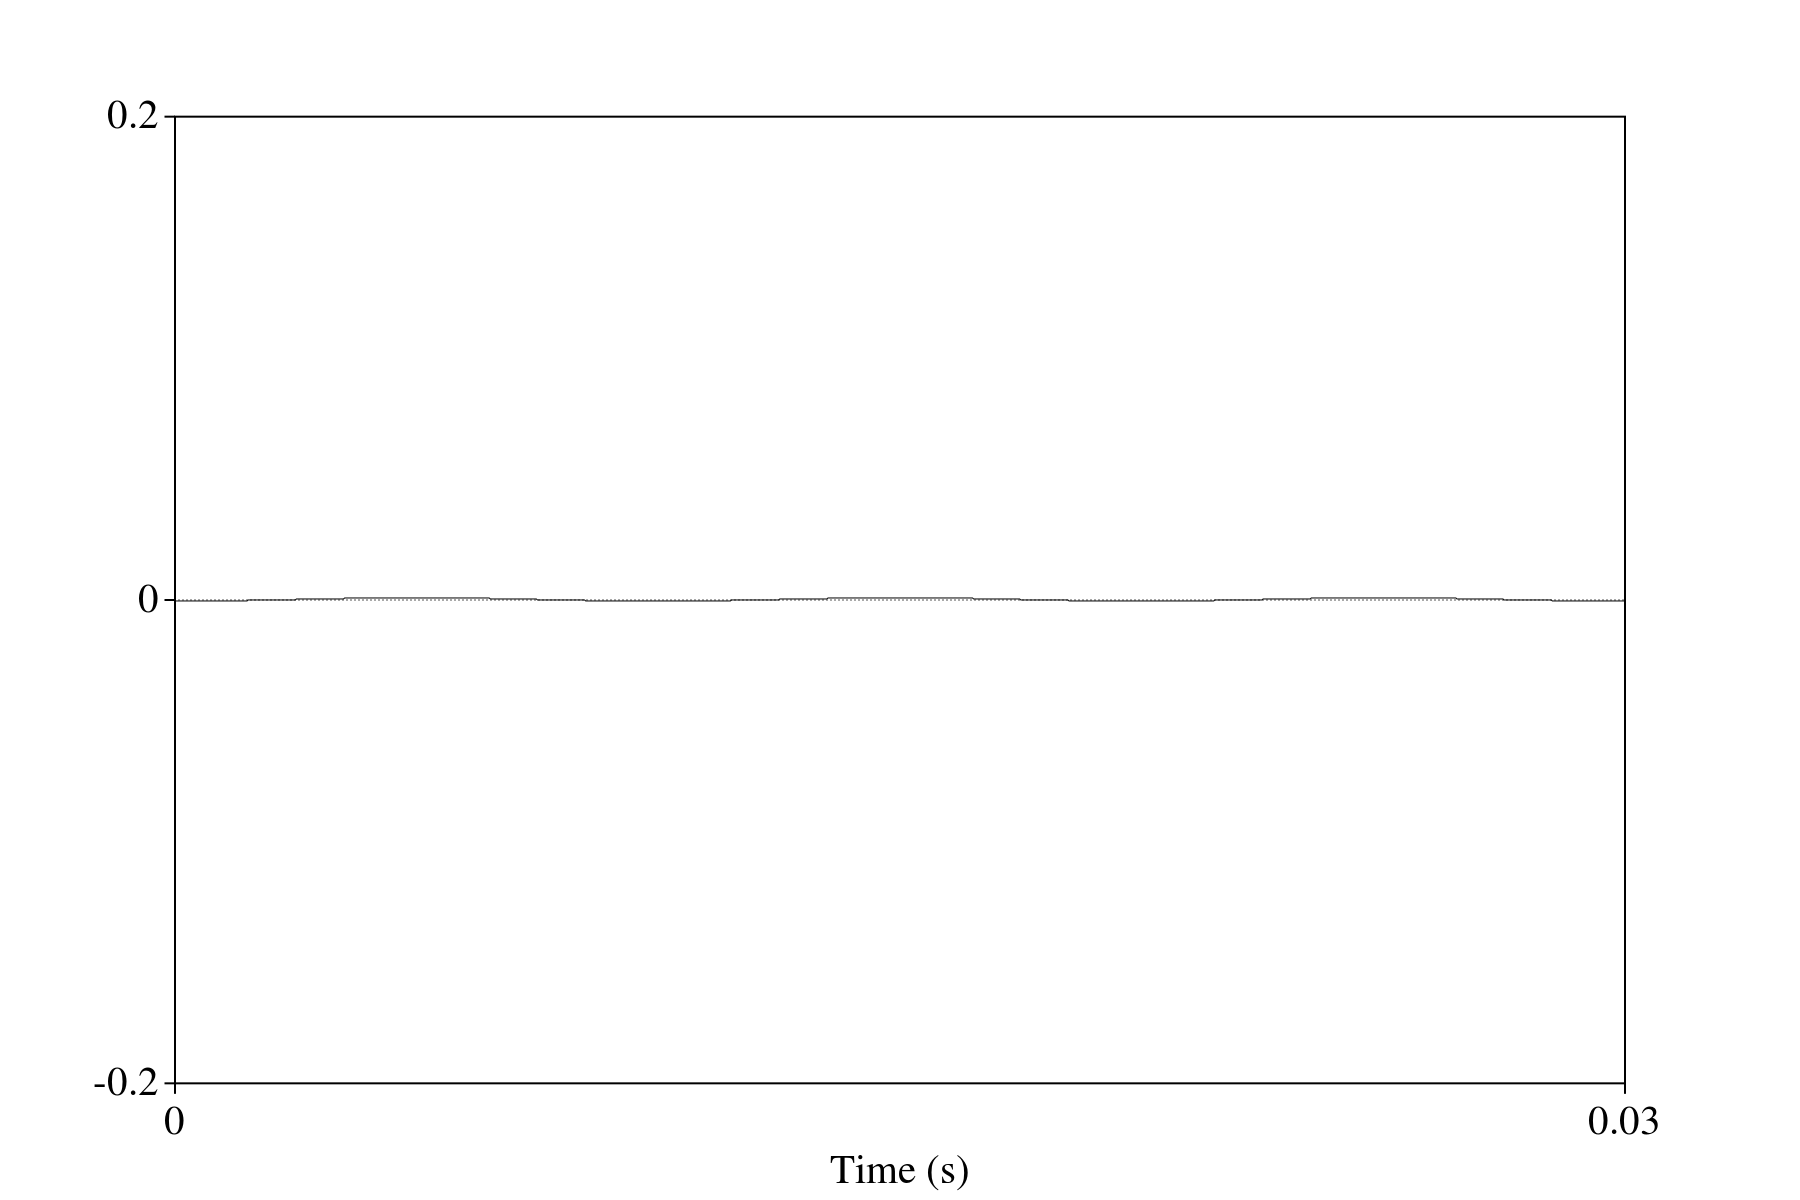
\includegraphics[width=\textwidth]{figure/wave-out-of-phase-added.png}
  \caption{The sound wave resulting from the combination of the two out of phase waves in Fig. \ref{fig:wave-out-of-phase}.}
  \label{fig:wave-out-of-phase-added}
\end{subfigure}
\caption{Demonstration of the combination of two completely out-of-phase waves with the same amplitude and frequency.}
\end{figure}

In order for this complete negation to happen, the two waves need to be coming from opposite directions toward one another.  Of course, it is not very often that two waves of the exact same frequency and amplitude, with exactly opposing phase, meet in such a way to completely negate.  However, varying degrees of negation occur frequently due to phase.  For example, if the 100 Hz wave from Figure \ref{fig:sound-wave-addition} were combined with a 200Hz wave with a slightly shifted phase, a different wave would be produced, seen in Figure \ref{fig:sound-combined-shifted-phase}.  

\begin{figure}[h!]
\begin{subfigure}{0.5\textwidth}
  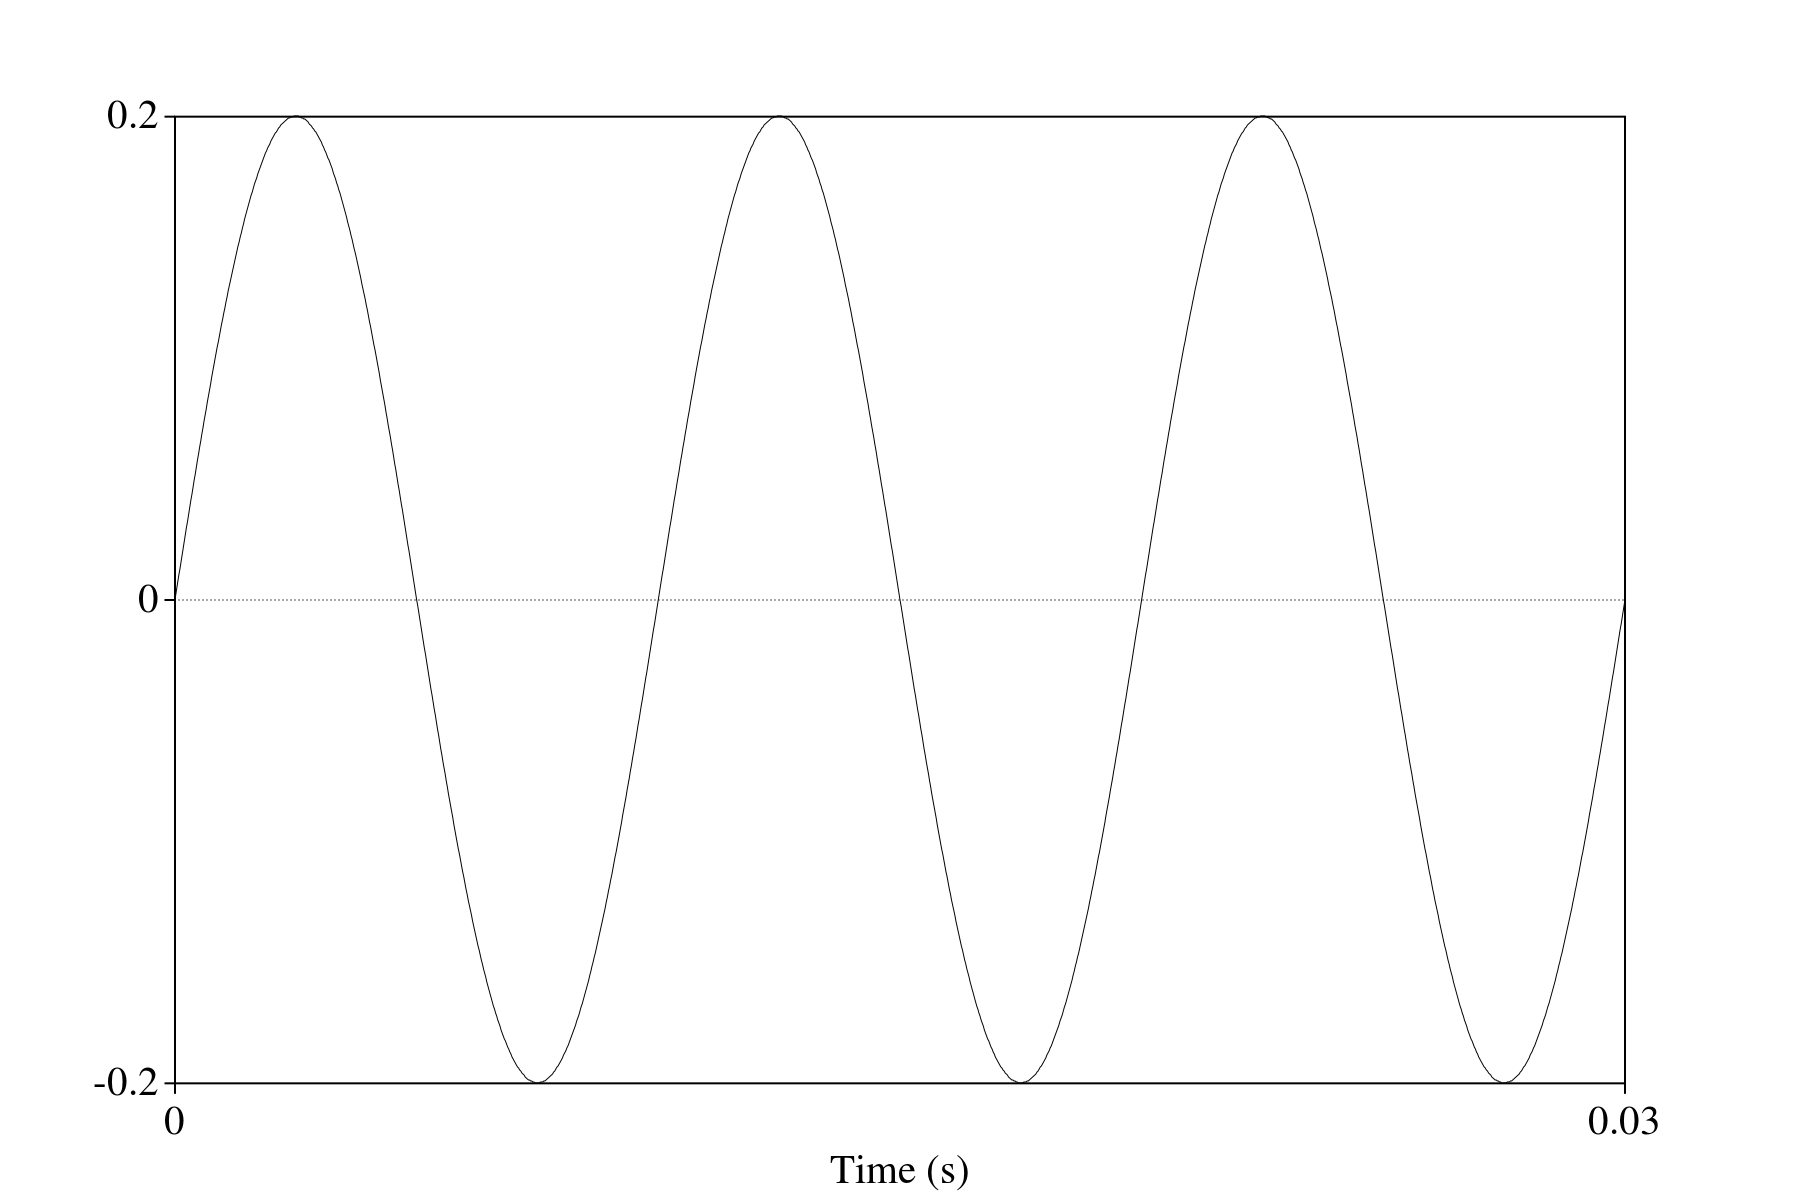
\includegraphics[width=\textwidth]{figure/basic-sound-wave.png}
  \caption{Two sound waves with frequency of 100 Hz and the same amplitude, completely out of phase.}
  \label{fig:wave-out-of-phase}
\end{subfigure}
\qquad
\begin{subfigure}{0.5\textwidth}
  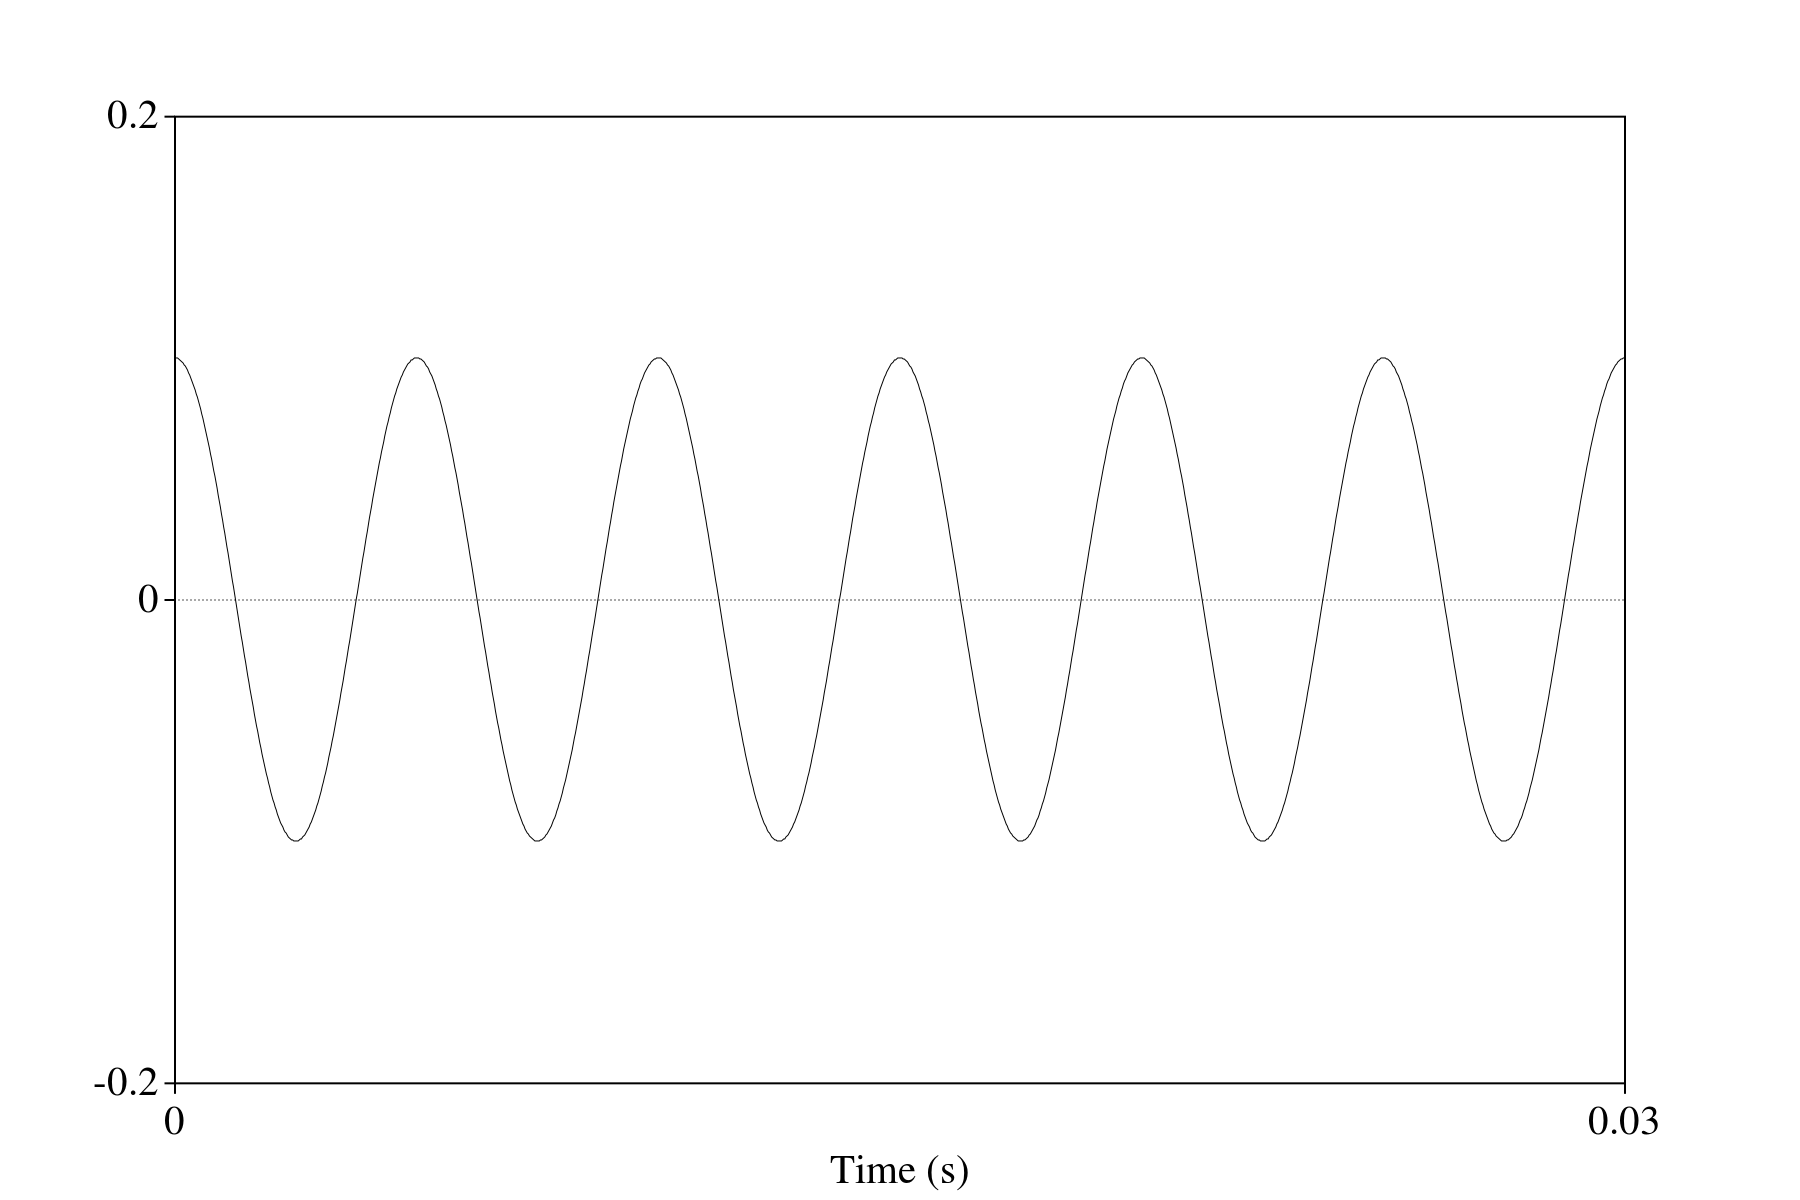
\includegraphics[width=\textwidth]{figure/sound-wave-addition-200hz-shifted.png}
  \caption{The sound wave resulting from the combination of the two out of phase waves in Fig. \ref{fig:wave-out-of-phase}.}
  \label{fig:wave-addition-200hz-shifted}
\end{subfigure}
%
\begin{center}
\begin{subfigure}{0.5\textwidth}
  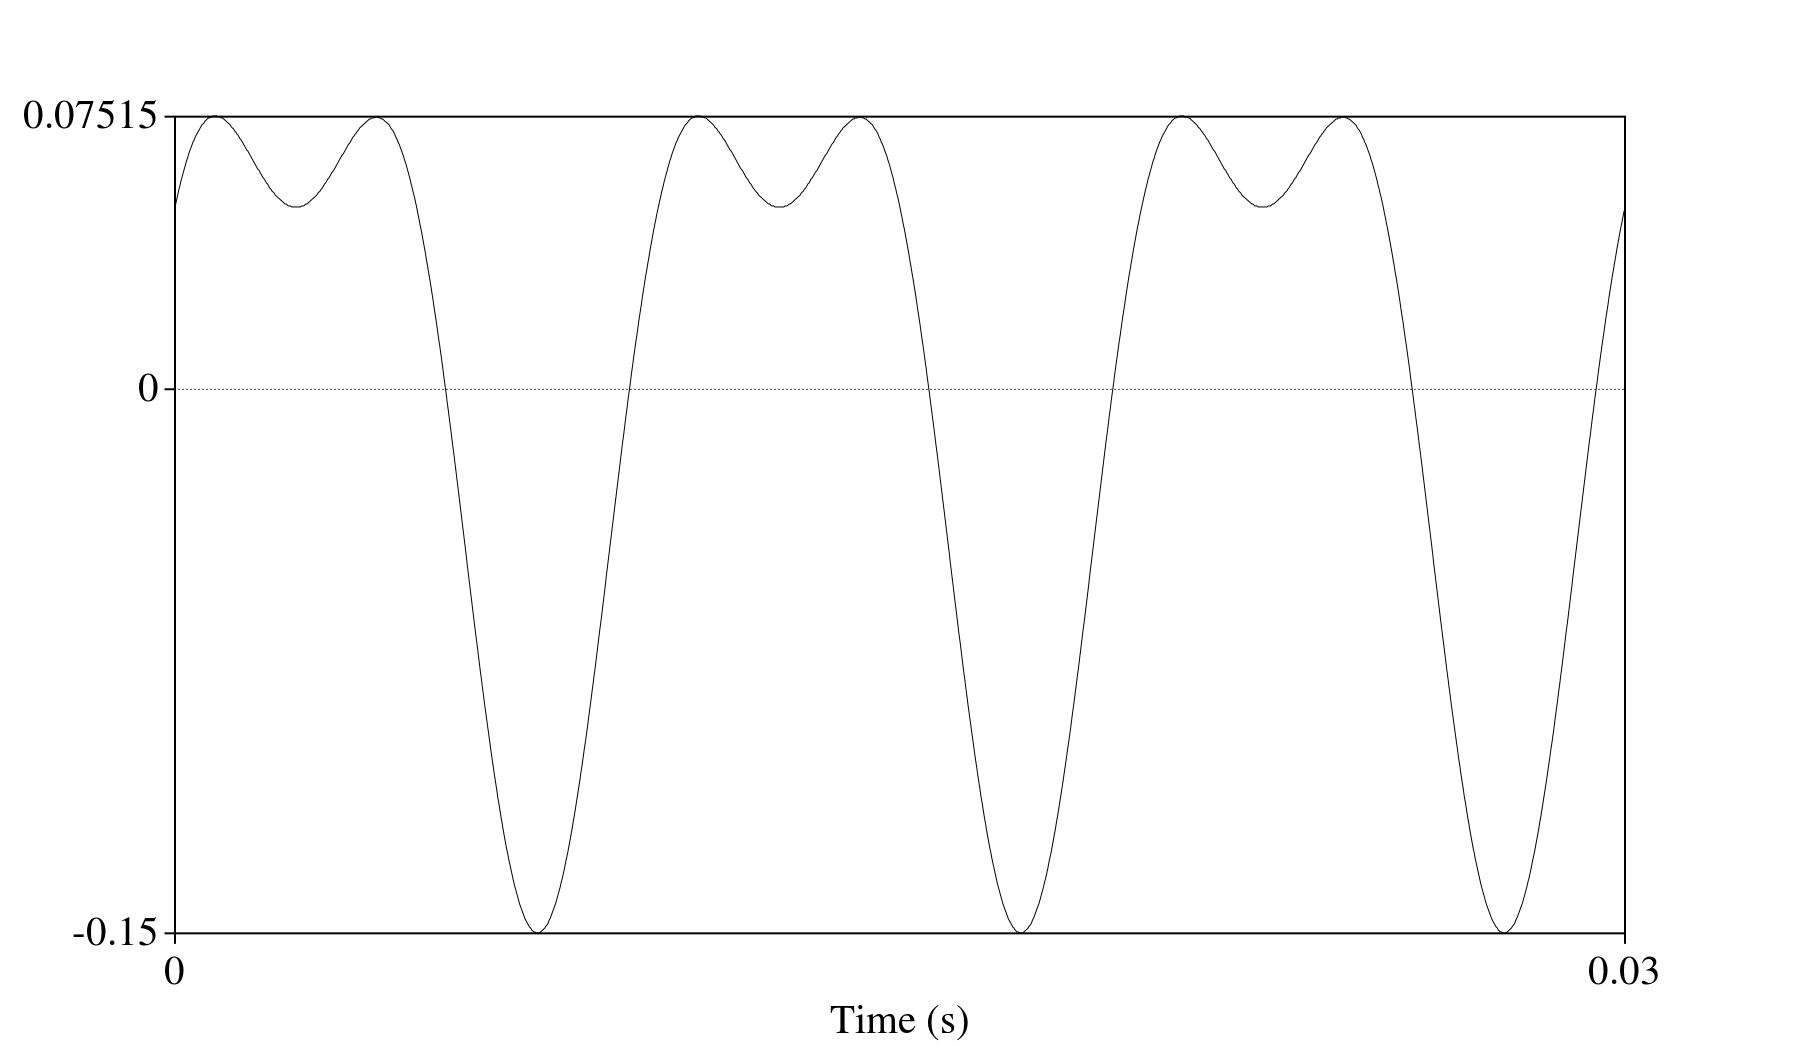
\includegraphics[width=\textwidth]{figure/sound-combined-shifted-phase.png}
  \caption{The sound wave resulting from the combination of the two out of phase waves in Fig. \ref{fig:wave-out-of-phase}.}
  \label{fig:sound-combined-shifted-phase}
\end{subfigure}
\end{center}
\caption{Demonstration of the combination of the same two waves as in Fig. \ref{fig:sound-wav-addition}, where the phase of the 200 Hz wave in Fig. \ref{fig:sound-wave-B} was shifted slightly (cf. Fig. \ref{fig:wave-addition-200hz-shifted})}
\label{fig:sound-shifted-phase}
\end{figure}

The combination of waves from multiple sound sources increases greatly in complexity as the number of sources increases, and the sounds originating from the sources are complex (ie. containing multiple frequency elements), such as speech.  Speech rarely occurs in isolation from from all external sound, yet we are still to largely understand speech in everyday environments; for example it is generally easy for humans to understand the speech of an interlocutor while sitting on a bench at a park.

The auditory system is actually quite skilled at identifying separate sources, even complex ones, like speech. Despite the shifted phase in Figure \ref{fig:sound-shifted-phase}, the human auditory system would still be able to detect and identify two separate waves.  While it undoubtedly plays a part, the differences in phase of combined signals does not normally completely negate a signal, nor render it unintelligible.  It is for this reason, and the complexity of phase calculations, that most efforts to remove speech from noise ignore the phase component.

\subsection{Difficulties of Speech in Noise}

Nevertheless, there are still situations in which it is difficult to parse speech in noise.  This is most often due to signals with energy at similar frequencies that overlap.  The greater the amplitude of a signal at frequencies overlapping with those of speech, the more difficult the speech will be to understand.  This can be visualized in the spectrograms of the sentence ``A rich farm is rare in this sandy waste.'' in Figure \ref{fig:signal-SNR-intro}.  In Figure \ref{fig:signal-SNR-intro-high}, the amplitude, or loudness, of the noise is well below that of speech; one would likely easily understand this speech.  However, Figure \ref{fig:signal-SNR-intro-low} has a much greater noise level compared to speech.

\begin{figure}[h!]
\centering
\begin{subfigure}{0.75\textwidth}
  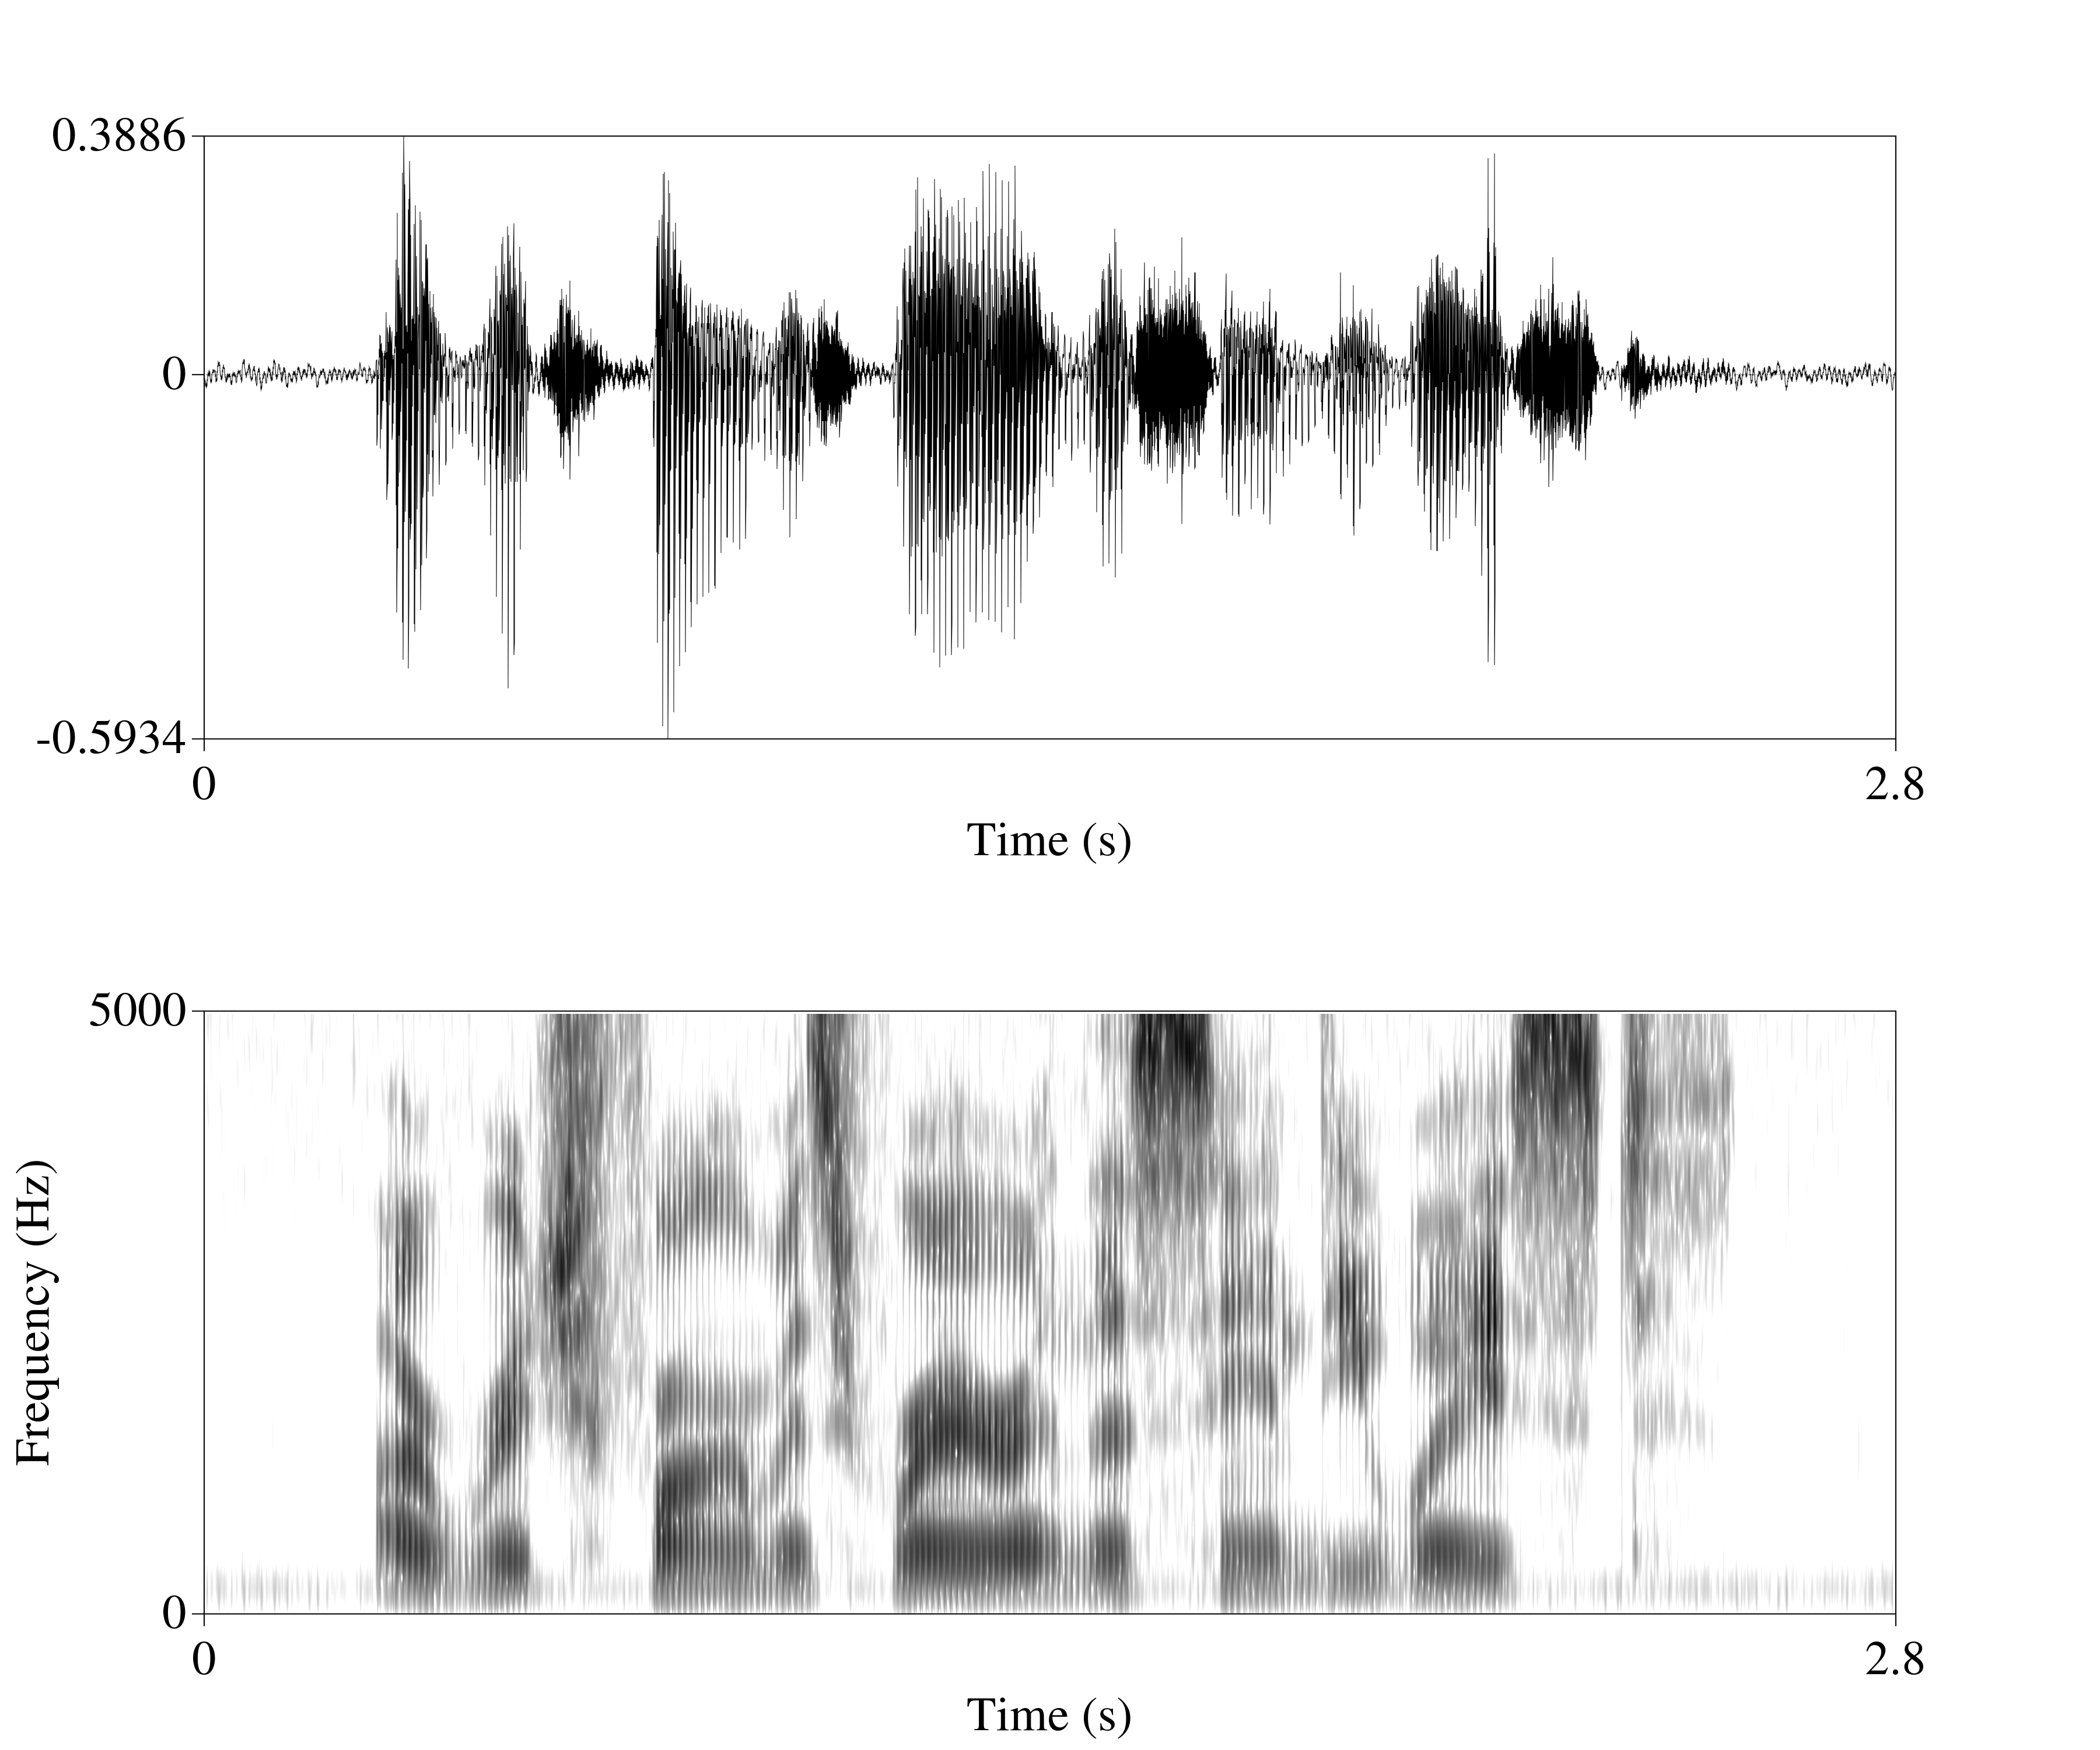
\includegraphics[width=.9\textwidth]{figure/signal-SNR-intro-high.png}
  \caption{A sentence spoken with a low level of background noise, resulting in a \textit{high} SNR.}
  \label{fig:signal-SNR-intro-high}
\end{subfigure}
%
\begin{subfigure}{0.75\textwidth}
  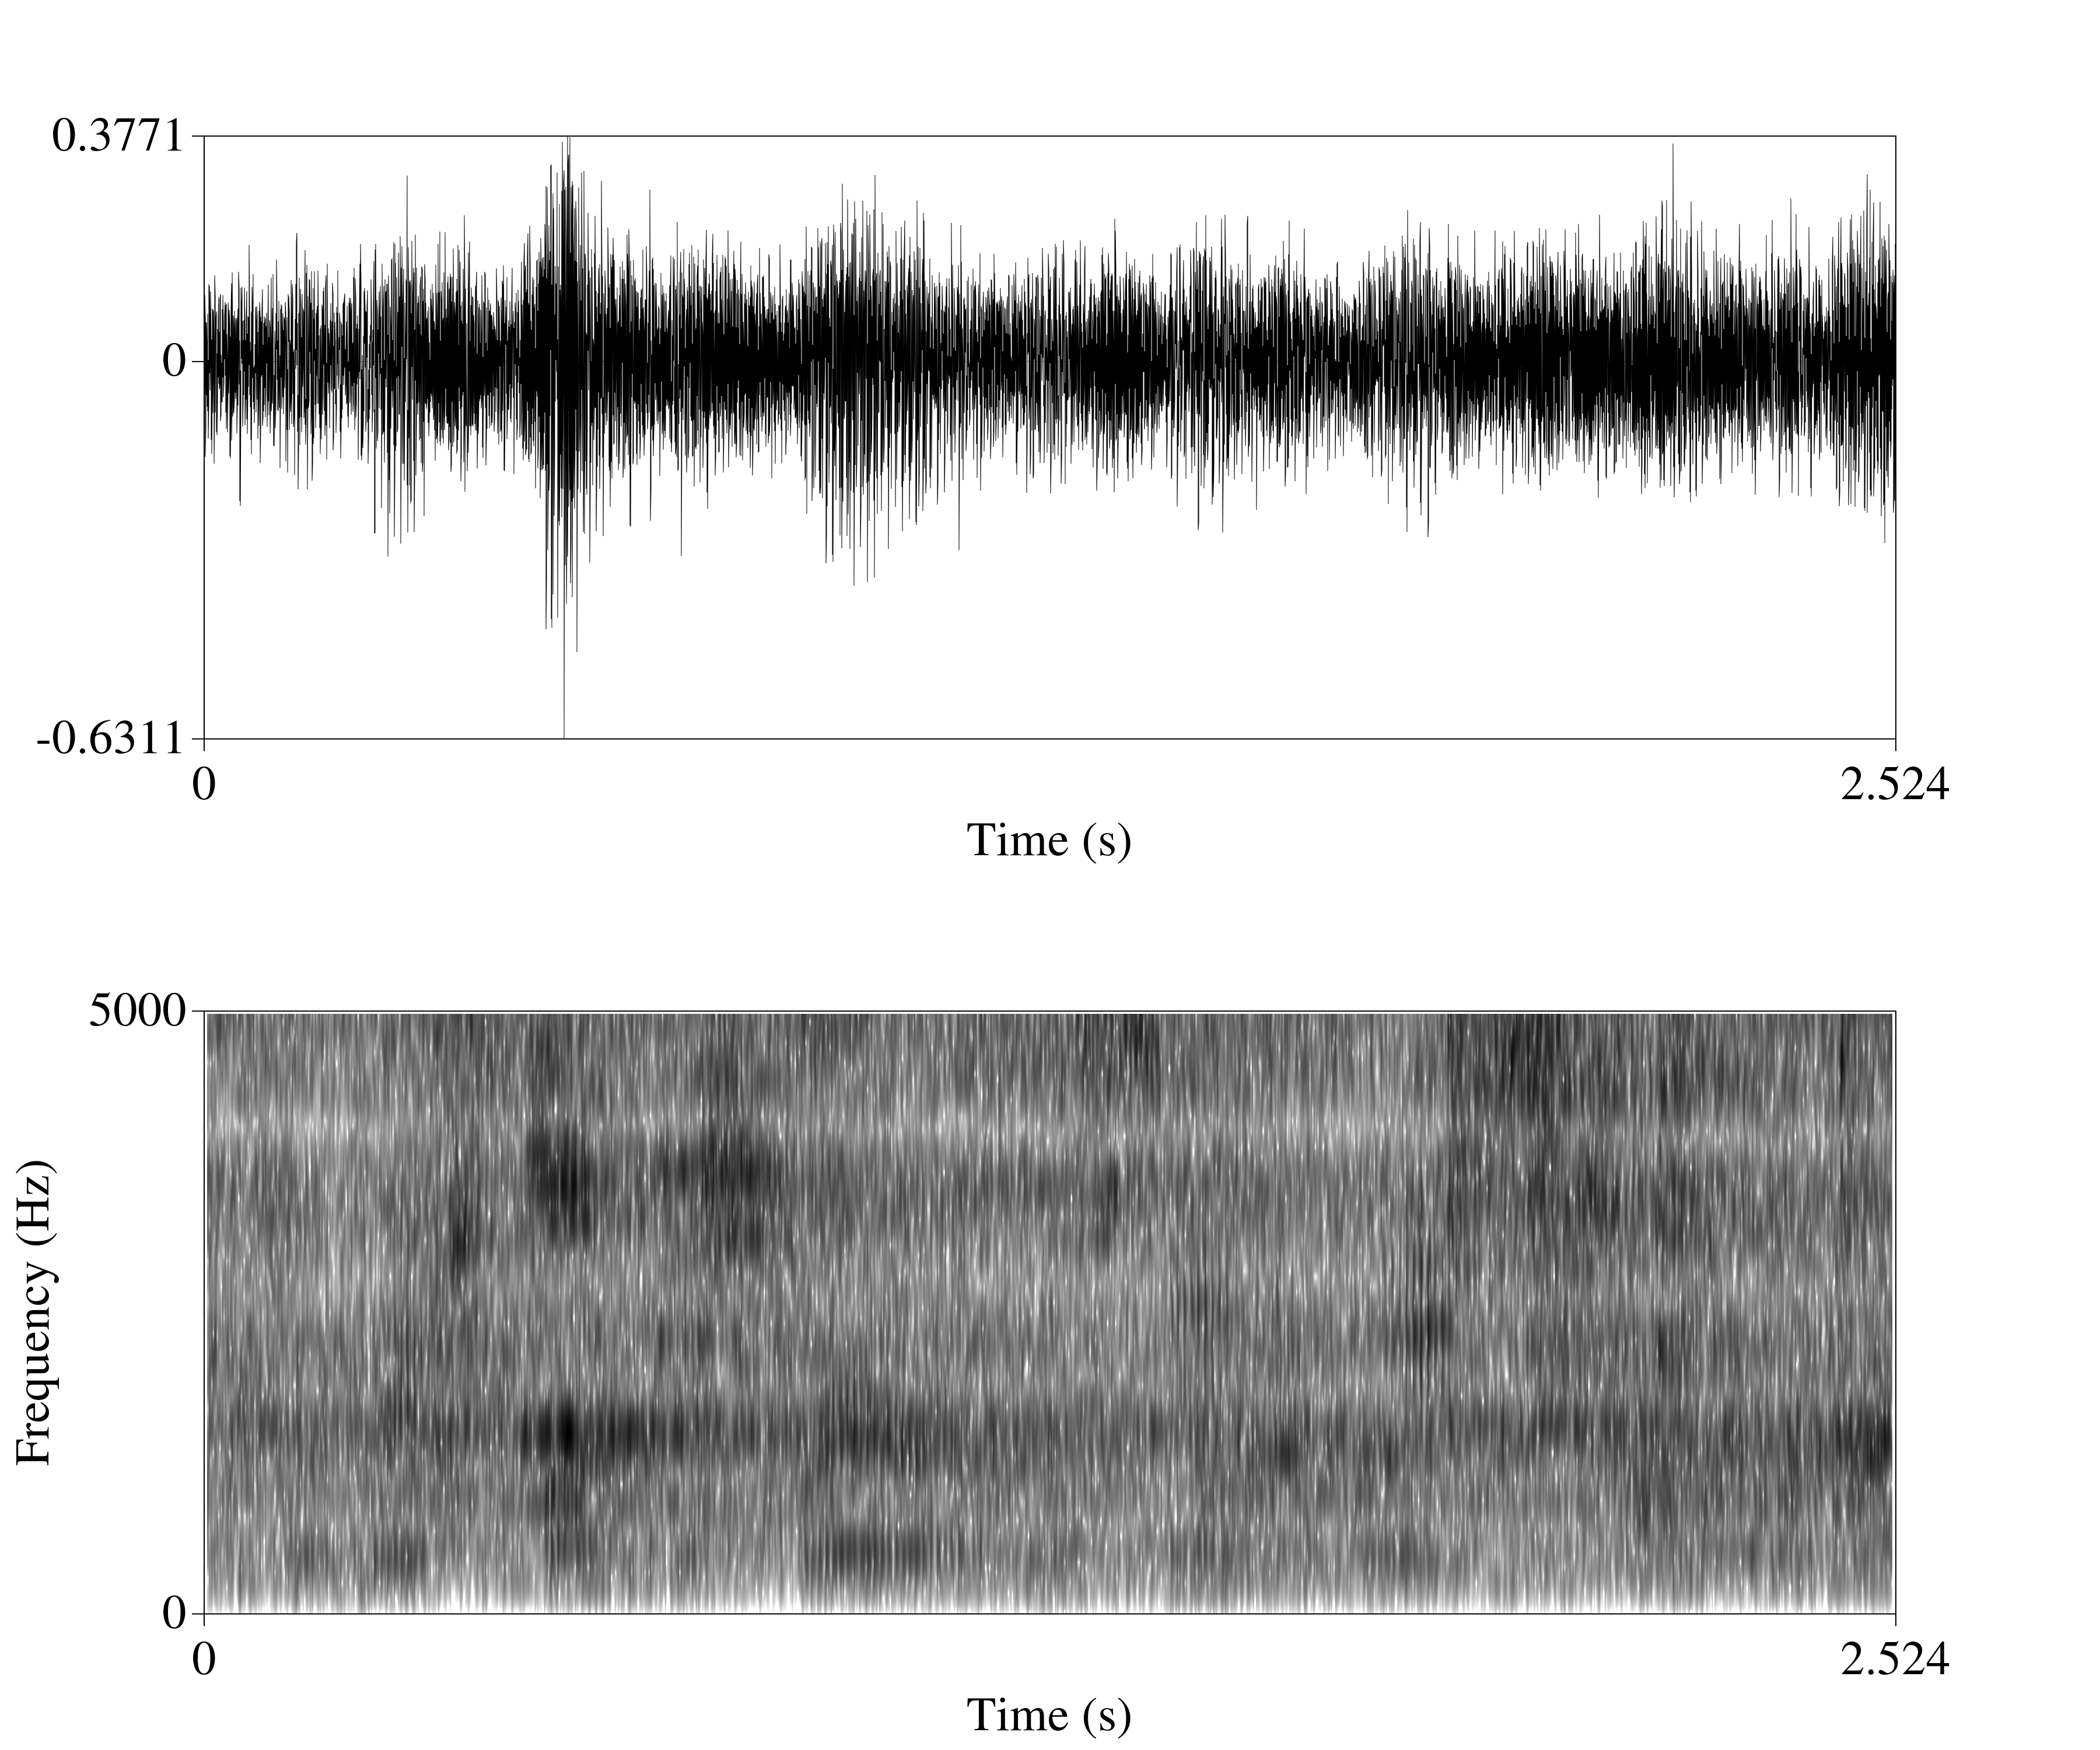
\includegraphics[width=.9\textwidth]{figure/signal-SNR-intro-low.png}
  \caption{A sentence spoken with a high level of background noise, resulting in a \textit{low} SNR.}
  \label{fig:signal-SNR-intro-low}
\end{subfigure}
\caption{Waveforms and spectrograms of the sentence ``A rich farm is rare in this sandy waste''.}
\label{fig:signal-SNR-intro}
\end{figure}

This relationship between speech and any background noise is called the signal to noise ration (SNR).  A complex signal with a higher signal to noise ratio (cf. Fig \ref{fig:signal-SNR-intro-high}) is generally easier to understand, because the amplitude of the speech (the `signal' of interest) is much greater than that of the noise.  Consequently a lower SNR (cf. Fig. \ref{fig:signal-SNR-intro-low}) results in speech that is more difficult to understand, because the amplitude of the speech is close to - or below - the amplitude of the background noise.

This poses a problem for human listeners, but generally is more difficult to deal with in automatic speech recognition (ASR), since the electronic device does not contain a highly-skilled, built-in auditory cortex.  There are a number of ways which have been proposed to deal with noise in a speech signal, both for human and automatic speech recognition.  These will be discussed further in Chapters 3\ref{chapter3} and 4\ref{chapter4}.

\section{Overview of Dissertation}\label{ch1:diss-overview}

This report aims to explore a novel method of human speech perception and automatic speech recognition (ASR) in noisy environments.  The method proposes that speech be recorded from the inside of the ear canal of the speaker, and slightly transformed, sent to the human hearer or the computer receiver for recognition.  By collecting speech from the ear, it allows for usage of the human skull and adjacent tissues to passively filter out the noisy environment, leaving only - or mostly - the human speech carrying the intended message.  
	
The intention of this study is to determine a) if recording human speech from the inside of the ear canal can significantly reduce background noise in a signal, b) if intelligible speech, suitable for communication, can be collected from the inside of the ear canal, c) if humans find speech recorded from the ear canal more intelligible than speech in noisy conditions, and finally d) if ASR systems are able to recognize speech recorded in the ear canal with greater accuracy than speech recorded in noise.
	
Since currently there is no established corpus of data that contain speech recorded from the inside of the ear canal together with speech simultaneously recorded from the mouth in noisy environments, it was necessary to record speakers in this environment and create a new corpus.  The theory behind the acoustics of recording speech from the ear canal, as well as the process for developing this corpus are described in Chapter 2\ref{chapter2}, along with a discussion of the recorded speech.  Chapter 3\ref{chapter3} will outline a human perception experiment, tasking listeners with the transcription of various sentences of speech recorded at the mouth in noise in noise, and recorded from the ear.   Chapter 4\ref{chapter4} describes the use of this same speech with an ASR system, and its recognition performance.  Chapter 5\ref{chapter5} will summarize the previous chapters and engage in an overall discussion of the implications of the results, the limitations of the present experiments and methods, and suggestions for future research direction.


\bibliographystyle{apa}
\bibliography{DissRefs.bib}
\end{document}
